\documentclass[12pt]{article}
\usepackage{preamble}
\begin{document}

%%%%%%%%%%%%%%%%%frond page%%%%%%%%%%%%%%%%%%%%%%%%%%%%%%%%%%
\begin{titlepage}
\title{Firms' Carbon Emissions and Stock Returns}
\author{Giacomo Morelli\thanks{Department of Statistical Sciences, Sapienza University of Rome} \and 
Cong Wang\thanks{Department of Economics and Law, Sapienza University of Rome}}
\date{\today}
\maketitle
\begin{abstract}
\noindent In recent years, unanticipated climate change risks have propelled green portfolios to achieve superior returns compared to their brown counterparts. Paradoxically, both empirical and theoretical evidence underscore a perplexing phenomenon: brown firms, characterized by higher carbon emissions or lower ESG (Environmental, Social, and Governance) scores, tend to yield greater expected stock returns. The discrepancy is primarily attributed to investors' demand for climate change-related risk premiums from these brown firms' stocks. This paper seeks to explore such an apparent contradiction. Despite the consistent outperformance of green portfolios over their brown counterparts, empirical studies at the firm level frequently uncover the reverse trend. By conducting empirical analyses encompassing all publicly listed companies in the U.S. stock market spanning the years 2002 to 2021, our objective is to furnish a comprehensive explanation for this intriguing and seemingly contradictory disparity.
\\
\vspace{0in}\\
\noindent\textbf{Keywords:} Carbon Emission, Stock Return, Climate Concerns\\
\vspace{0in}\\
\noindent\textbf{JEL Codes:} G11, G12, G30\\
\bigskip
\end{abstract}
\setcounter{page}{0}
\thispagestyle{empty}
\end{titlepage}
\pagebreak \newpage

\doublespacing

%%%%%%%%%%%%%%%%%%%%%%%%%%%%%%%%%%%%%%%%%%%%%%%%%%%%%%%%%%%%%%%%
%%%%%%%%%%%%%%%%%%%%%%%%%%%%%%%%%%%%%%%%%%%%%%%%%%%%%%%%%%%%%%%%
\section{Introduction} \label{sec:introduction}
%%%%%%%%%%%%%%%%%%%%%%%%%%%%%%%%%%%%%%%%%%%

In the face of mounting challenges such as geopolitical conflictions, pandemics, and global warming, the call for sustainable investment and environmentally responsible production has never been more urgent. These pressing global concerns have underscored the critical need to prioritize sustainability as a central tenet of our collective future. In addressing these challenges, the United Nations has published \cite{fund2015sustainable} which comprises 17 interlinked objectives that emphasize the intricate connections between environmental, social, and economic aspects of sustainable development. \cite{alliance2017global} states that by 2016, the total value of assets being professionally managed under responsible investment strategies worldwide had surged to a staggering \$22.89 trillion. This remarkable figure represented a substantial increase of 25 percent since 2014, underscoring the growing momentum behind sustainable and socially responsible investment practices on a global scale right after the Paris \cite{agreement2015paris}.

Investors frequently turn to ESG (Environmental, Social, and Governance) scores when evaluating companies to gauge their environmental, social and governance practices, especially the E scores for environment. These scores play an important role in categorizing companies into "Green" and "Brown", signifying their commitment to sustainable practices or their lack thereof. However, a notable challenge arises from the fact that multiple ESG rating agencies, such as MSCI ESG Ratings, Sustainalytics, Bloomberg, among others, operate concurrently. Each of these agencies employs distinct valuation metrics and methodologies, leading to divergent ESG ratings for the same companies. In fact, recent research, as highlighted by \cite{avramov2022sustainable}, has revealed that this variation in ESG assessments can introduce uncertainty into the market. Such uncertainty has the potential to increase market premiums and diminish demand for the related stocks that exhibit higher ESG uncertainty, and create a complex landscape for investors to navigate. To circumvent the challenges associated with rating uncertainty, this paper adopts a pragmatic approach by relying on a single, yet robust, indicator to gauge companies' environmental performance: CO2 emissions. Carbon emissions are recognized as a primary driver of global warming, and they are mandated for disclosure by various stakeholders, including the Securities and Exchange Commission (SEC), investors, and the media. By focusing on this widely accepted and easily measurable metric, this study seeks to provide a clear and unambiguous assessment of firms' greenness and stock returns. 

This paper investigates whether firms characterized as "Green" due to their lower carbon emissions experience higher stock returns in comparison to "Brown" firms. The dataset utilized in this study encompasses all publicly traded stocks in the U.S. stock market from 2002 to 2021. The initial phase of this research involves an exploratory analysis of the relationship between firms' carbon emissions and their stock returns. Across the entire dataset, we categorize all the observations into percentiles based on total CO2 emissions, subsequently computing the average stock return within each percentile. The findings consistently reveal that stocks situated in the lower percentiles consistently exhibit higher average stock returns, with a decline in returns observed as percentiles progress toward the 100th percentile. Remarkably, this pattern persists when we consider different scopes of carbon emissions. It's worth noting that while one might attribute this trend to the size of firms, as carbon emissions tend to be positively correlated with firm size, our analysis does not reveal a similar pattern between firm size and stock returns. Furthermore, we apply a similar methodology to examine the relationship between firms' stock returns and carbon intensity, which is defined as a firm's carbon emissions scaled by its revenue. This measure is a crucial proxy for a firm's carbon footprint in the current corporate finance literature. However, in contrast to our findings on carbon emissions, we do not identify a clear and consistent relationship between firms' stock returns and carbon intensity.

In recent years, the outperformance of Green portfolios over their Brown counterparts, attributed to unexpected climate concerns, has garnered significant attention. Notably, a study by \cite{pastor2022dissecting} employs firms' ESG scores to construct Green and Brown portfolios, revealing the existence of a "green premium" that rewards investments in environmentally responsible assets with higher ESG scores. In alignment with this methodology, we adopt a similar approach by constructing Green and Brown portfolios based solely on firms' carbon emissions. Each month, we categorize companies into three distinct groups: those with the lowest carbon emissions are designated as Green portfolios, those with higher emissions fall into Brown portfolios, and those with emissions ranking in the middle are classified as Neutral. Over the entire dataset spanning from 2002 to 2021, the Green portfolios have delivered impressive cumulative returns, exceeding 500\%, while their Brown counterparts achieved approximately 260\% in cumulative returns. However, when we replicate this approach using firms' carbon intensity to construct Green and Brown portfolios, the results diverge. In terms of cumulative returns, we find no clear evidence supporting the outperformance of Green portfolios; in fact, most of the time, Brown portfolios exhibit higher cumulative returns. By the end of the sample period, both Green and Brown portfolios reach cumulative returns of around 300\%. These findings shed light on the nuanced relationship between carbon emissions and stock returns, highlighting the multifaceted nature of sustainable investing.

Through a comprehensive regression analysis, we unearth intriguing insights into the performance of Green and Brown portfolios based on different criteria. When considering firms' total carbon emissions, Green portfolios exhibit a statistically significant monthly outperformance of 44.3 basis points over their Brown counterparts. However, when evaluating portfolios constructed based on carbon intensity, the difference between Green and Brown portfolios narrows to a mere 0.4 basis points, with no statistical significance observed. Delving deeper into the analysis, we apply the Fama-French 5 factors model to regress the Green minus Brown (GMB) portfolios. An intriguing finding emerges in the form of a significant intercept that defies explanation, suggesting the presence of an unaccounted-for factor, possibly the Green minus Brown factor discussed by \cite{pastor2022dissecting}. 

Another paper by \cite{pastor2021sustainable} posits that Green portfolios outperform Brown in the presence of unexpected climate change-related concerns. To further illuminate this relationship, we leverage the Media Climate Change Concern (MCCC) index developed by \cite{ardia2022climate} and employ an ARX model to compute the Unexpected Media Climate Change Concerns (UMC). The regression results reveal a positive relationship between UMC and GMB portfolios. Specifically, a 1-unit increase in UMC corresponds to a 1.49\% increase in the return of GMB portfolios, with statistical significance observed at the 1\% level. Moreover, when we conduct separate regressions of the UMC index on Green and Brown portfolios, distinct patterns emerge. The coefficient on Brown portfolios stands at -1.27, signifying that in periods of elevated unexpected climate risk, the return for Brown portfolios experiences a notable decline. In contrast, the coefficient of the UMC index on Green portfolios is positive at 0.23, indicating that a higher UMC index is associated with higher returns for Green portfolios. Remarkably, the UMC index does not exhibit statistical significance concerning the return of Neutral portfolios, highlighting the selective impact of unexpected climate concerns on the investment performance of different portfolios.

In our aggregated portfolio analysis, our findings align with \cite{pastor2022dissecting}, suggesting that Green portfolios, which encompass firms with higher ESG scores or lower carbon emissions, tend to outperform their Brown counterparts. These results are corroborated by \cite{friede2015esg}, who also indicate that Green firms often exhibit better financial performance. However, when we delve into firm-level analyses, as conducted by \cite{bolton2021investors} and \cite{aswani2023carbon}, a stark contradiction emerges. Their research suggests that firms with higher carbon emissions tend to yield higher stock returns, directly conflicting with our portfolio performance findings.

To address this discrepancy, we shift our focus to firm-level data and employ panel Ordinary Least Squares (OLS) regression to explore the relationship between firms' total carbon emissions and stock returns. Recognizing the presence of unobserved time-variant factors and time-invariant industry-specific factors, we incorporate Industry + Time fixed effects in our panel regression model. Our results reveal a positive correlation between firms' stock returns and total carbon emissions indicating that firms with higher CO2 emissions tend to have higher stock returns on average, yet this relationship lacks statistical significance. 

The choice to incorporate Industry + Time two-way fixed effects is rooted in the assumption that there exist unobserved time-variant factors linked to time periods and time-invariant factors associated with industries. This assumption hinges on the belief that firms within the same industry exhibit similar stock return behaviors. A more stringent assumption is that even in the same industry firms' stock returns still behave differently, due to some idiosyncratic characteristics associated with each specific firm. Under this new assumption, we apply Entity + Time two-way fixed effects. The results of this analysis reveal a significant and negative relationship between firms' carbon emissions and stock returns, both statistically and economically. Specifically, a 1\% increase in firms' total carbon emissions corresponds to a 0.66\% decrease in stock returns, on average. These findings provide robust support for the notion that higher carbon emissions are associated with lower stock returns alongside our portfolio analysis, emphasizing the importance of accounting for idiosyncratic firm-level characteristics in our analysis. In our robustness analysis, we systematically vary the fixed effects and cluster standard errors at different levels. Notably, whenever we incorporate entity-fixed effects into the model, our findings consistently align with those of our benchmark model. This robustness underscores the reliability and stability of our results across various specifications, affirming the significance of entity-fixed effects in our analysis

In line with \cite{pastor2021sustainable}, who developed an equilibrium model based on ESG scores and stock returns, our firm-level analysis delves into the relationship between firms' carbon emissions, unexpected climate change concerns, and stock returns. We find that when unexpected climate change concerns materialize, brown firms characterized by higher total CO2 emissions tend to experience decreases in their stock returns. Importantly, these results hold true across various sets of control variables containing macroeconomic conditions. After accounting for factors such as the Fama-French 5 factors, the investor sentiment index, the CFNAI index, WTI, and VIX, the intersection between firms' total carbon emissions and unexpected climate concerns remains significant, demonstrating a negative impact on stock returns, and the statistical significance is observed at the 1\% level. This robustness reinforces the link between firms' carbon emissions and stock performance in the face of climate change concerns. When unexpected climate change concerns hit the economy, firms with higher carbon emissions (Brown Firms) experience losses in their stock returns. 

\subsection*{Related Literature}

Our study contributes to a vast empirical literature on sustainable investing, encompassing both aggregated portfolio and firm-level analyses. In a broader context, research in this field has gained significant momentum due to growing concerns about climate change and sustainability. For instance, \cite{krueger2020importance} conducted a study using survey data to investigate climate perception and found that climate risks, particularly those related to regulations, have started to materialize. Their research indicates that many investors, particularly those with a long-term perspective, larger portfolios, and a focus on ESG (Environmental, Social, and Governance) factors, prioritize risk management and engagement over divestment strategies. This underscores the evolving priorities and strategies of investors in response to climate-related challenges. 

Similarly, \cite{faccini2023dissecting} conducted groundbreaking research to assess whether market-wide physical or transition climate risks are priced into U.S. stocks. They found that only the climate-policy factor is priced, especially after 2012. Interestingly, their study revealed that investors seem to be less concerned about natural disasters, global warming, and decisions made at international climate summits. This research highlights the complexity of integrating climate risk into financial markets and the selective focus of investors on specific aspects of climate-related factors. 
		
In the midst of this dynamic landscape, our study adds to the body of knowledge by examining the relationship between firms' carbon emissions, climate change concerns, and stock returns. However, the current literature diverges when it comes to the performance of Green and Brown assets.  \cite{garvey2018carbon} have utilized carbon ratios to select stocks, revealing that lower carbon ratios are associated with higher stock returns and increased profitability. \cite{in2017being} constructed "Efficient-Minus-Inefficient" portfolios based on carbon intensity, demonstrating their ability to generate positive alpha since 2009. Meanwhile, \cite{andersson2016hedging} introduced a low carbon index, and find that when climate change mitigation is pending, the low carbon index performs the same as the benchmark, when carbon emission is priced, the index outperforms the benchmark. Additionally, \cite{hsu2023pollution} investigated the impact of toxic emissions intensity within industries, showcasing that the portfolio premium could not be explained by traditional factors, sentiment, political connections, or corporate governance, emphasizing the unique role of toxic emissions in stock returns. These studies all suggest that Green assets generate climate risk premiums, and outperform Brown assets especially when there is emission-related policy shocks.

Another branch of study declares that investors are already demanding compensation for carbon emission risk, hence Brown assets are associated with higher expected returns. Notably, studies like \cite{bolton2021investors} and \cite{aswani2023carbon} have found that firms with high CO2 emissions tend to yield higher stock returns, showcasing the influence of carbon intensity on investment choices for institutional investors, particularly in salient industries. \cite{baker2018financing} delved into the world of green bonds, which are used for environmentally sensitive purposes, and identified that green bonds are issued at a premium compared to otherwise similar ordinary bonds, highlighting investor demand for environmentally responsible investments. Meanwhile, \cite{zerbib2022sustainable} introduced the concept of exclusion premia, encompassing sin stocks, to elucidate the relationship between ESG factors and financial performance. They found that exclusion effects amounted to 2.79\% annually, with taste effects varying from -1.12\% to 0.14\%. Moreover, \cite{chava2014environmental} analyzed the impact of a firm's environmental profile on its cost of equity and debt capital, discovering that investors demanded significantly higher expected returns on stocks excluded by environmental screens compared to firms without such concerns. These excluded firms also exhibited lower institutional ownership and fewer banks participating in their loan syndicates. Additionally, \cite{bolton2021global} estimated the market-based premium associated with carbon risk at the firm level across 77 countries, uncovering a widespread carbon premium characterized by higher stock returns for companies with higher levels of carbon emissions. Lastly, \cite{gorgen2020carbon} found that Brown firms tended to yield higher average returns, while decreases in the greenness of firms were associated with lower announcement returns. However, when they constructed a carbon risk factor-mimicking portfolio, they did not find evidence of a carbon risk premium, emphasizing the complexity of the relationship between carbon risk and investment returns.

In response to the significant divergence between two contradictory branches of existing literature, this study adopts a comprehensive approach encompassing aggregated portfolio analysis and firm-level investigations. By bridging the gap and synthesizing findings from both approaches, we aim to provide a more holistic and nuanced understanding of the relationship between stocks' greenness, measured by their carbon emissions, and their corresponding stock returns.

\clearpage
%%%%%%%%%%%%%%%%%%%%%%%%%%%%%%%%%%%%%%%%%%%%%%%%%%%%%%%%%%%%%%%%
%%%%%%%%%%%%%%%%%%%%%%%%%%%%%%%%%%%%%%%%%%%%%%%%%%%%%%%%%%%%%%%%
%\section{Literature Review} \label{sec:literature review}
%\input{2. Literature review}
%\clearpage
%%%%%%%%%%%%%%%%%%%%%%%%%%%%%%%%%%%%%%%%%%%%%%%%%%%%%%%%%%%%%%%%
%%%%%%%%%%%%%%%%%%%%%%%%%%%%%%%%%%%%%%%%%%%%%%%%%%%%%%%%%%%%%%%%
%\section{Methodology} \label{sec:Methodology}
%\input{3. Methodology}
%\clearpage
%%%%%%%%%%%%%%%%%%%%%%%%%%%%%%%%%%%%%%%%%%%%%%%%%%%%%%%%%%%%%%%%
%%%%%%%%%%%%%%%%%%%%%%%%%%%%%%%%%%%%%%%%%%%%%%%%%%%%%%%%%%%%%%%%
\section{Data} \label{sec:data}
%%%%%%%%%%%%%%%%%%%%%%%%%%%%%%%%%%%%%%%%%%%%%%%%%%%
This research focuses exclusively on the U.S.-listed companies from 2002 to 2021. The dataset combines companies' carbon emission data from Trucost, financial accounting data from Compustat, and stock return data from CRSP (The Center for Research in Security Prices), all the datasets are linked using the CUSIP-PERMNO linkage table. The combined dataset encompasses 3,938 companies and a total of 480,119 observations. As depicted in Figure \ref{fig: num}, the graph presents the yearly count of both the number of companies and observations.

Notably, the carbon emission data collection began in 2002 with limited coverage. However, after 2015, there was a substantial surge in the number of companies included in the dataset. This remarkable expansion can be attributed to the effect of various international agreements that were signed during this period, such as the \textit{Addis Ababa Action Agenda} (AAAA), the \textit{Sendai Framework for Disaster Risk Reduction 2015-2030} (SFDRR), and \textit{The Paris Agreement on Climate Change}. These agreements, as discussed by \cite{engberg2021influence}, \cite{kelman2015climate}, and \cite{dimitrov2016paris}, have played an important role in addressing global climate challenges. They have particularly underscored the significance of sustainable development and initiatives to combat climate change.

\begin{figure}[!ht]
\centering
\caption{\textbf{Number of Firms and Observations}}
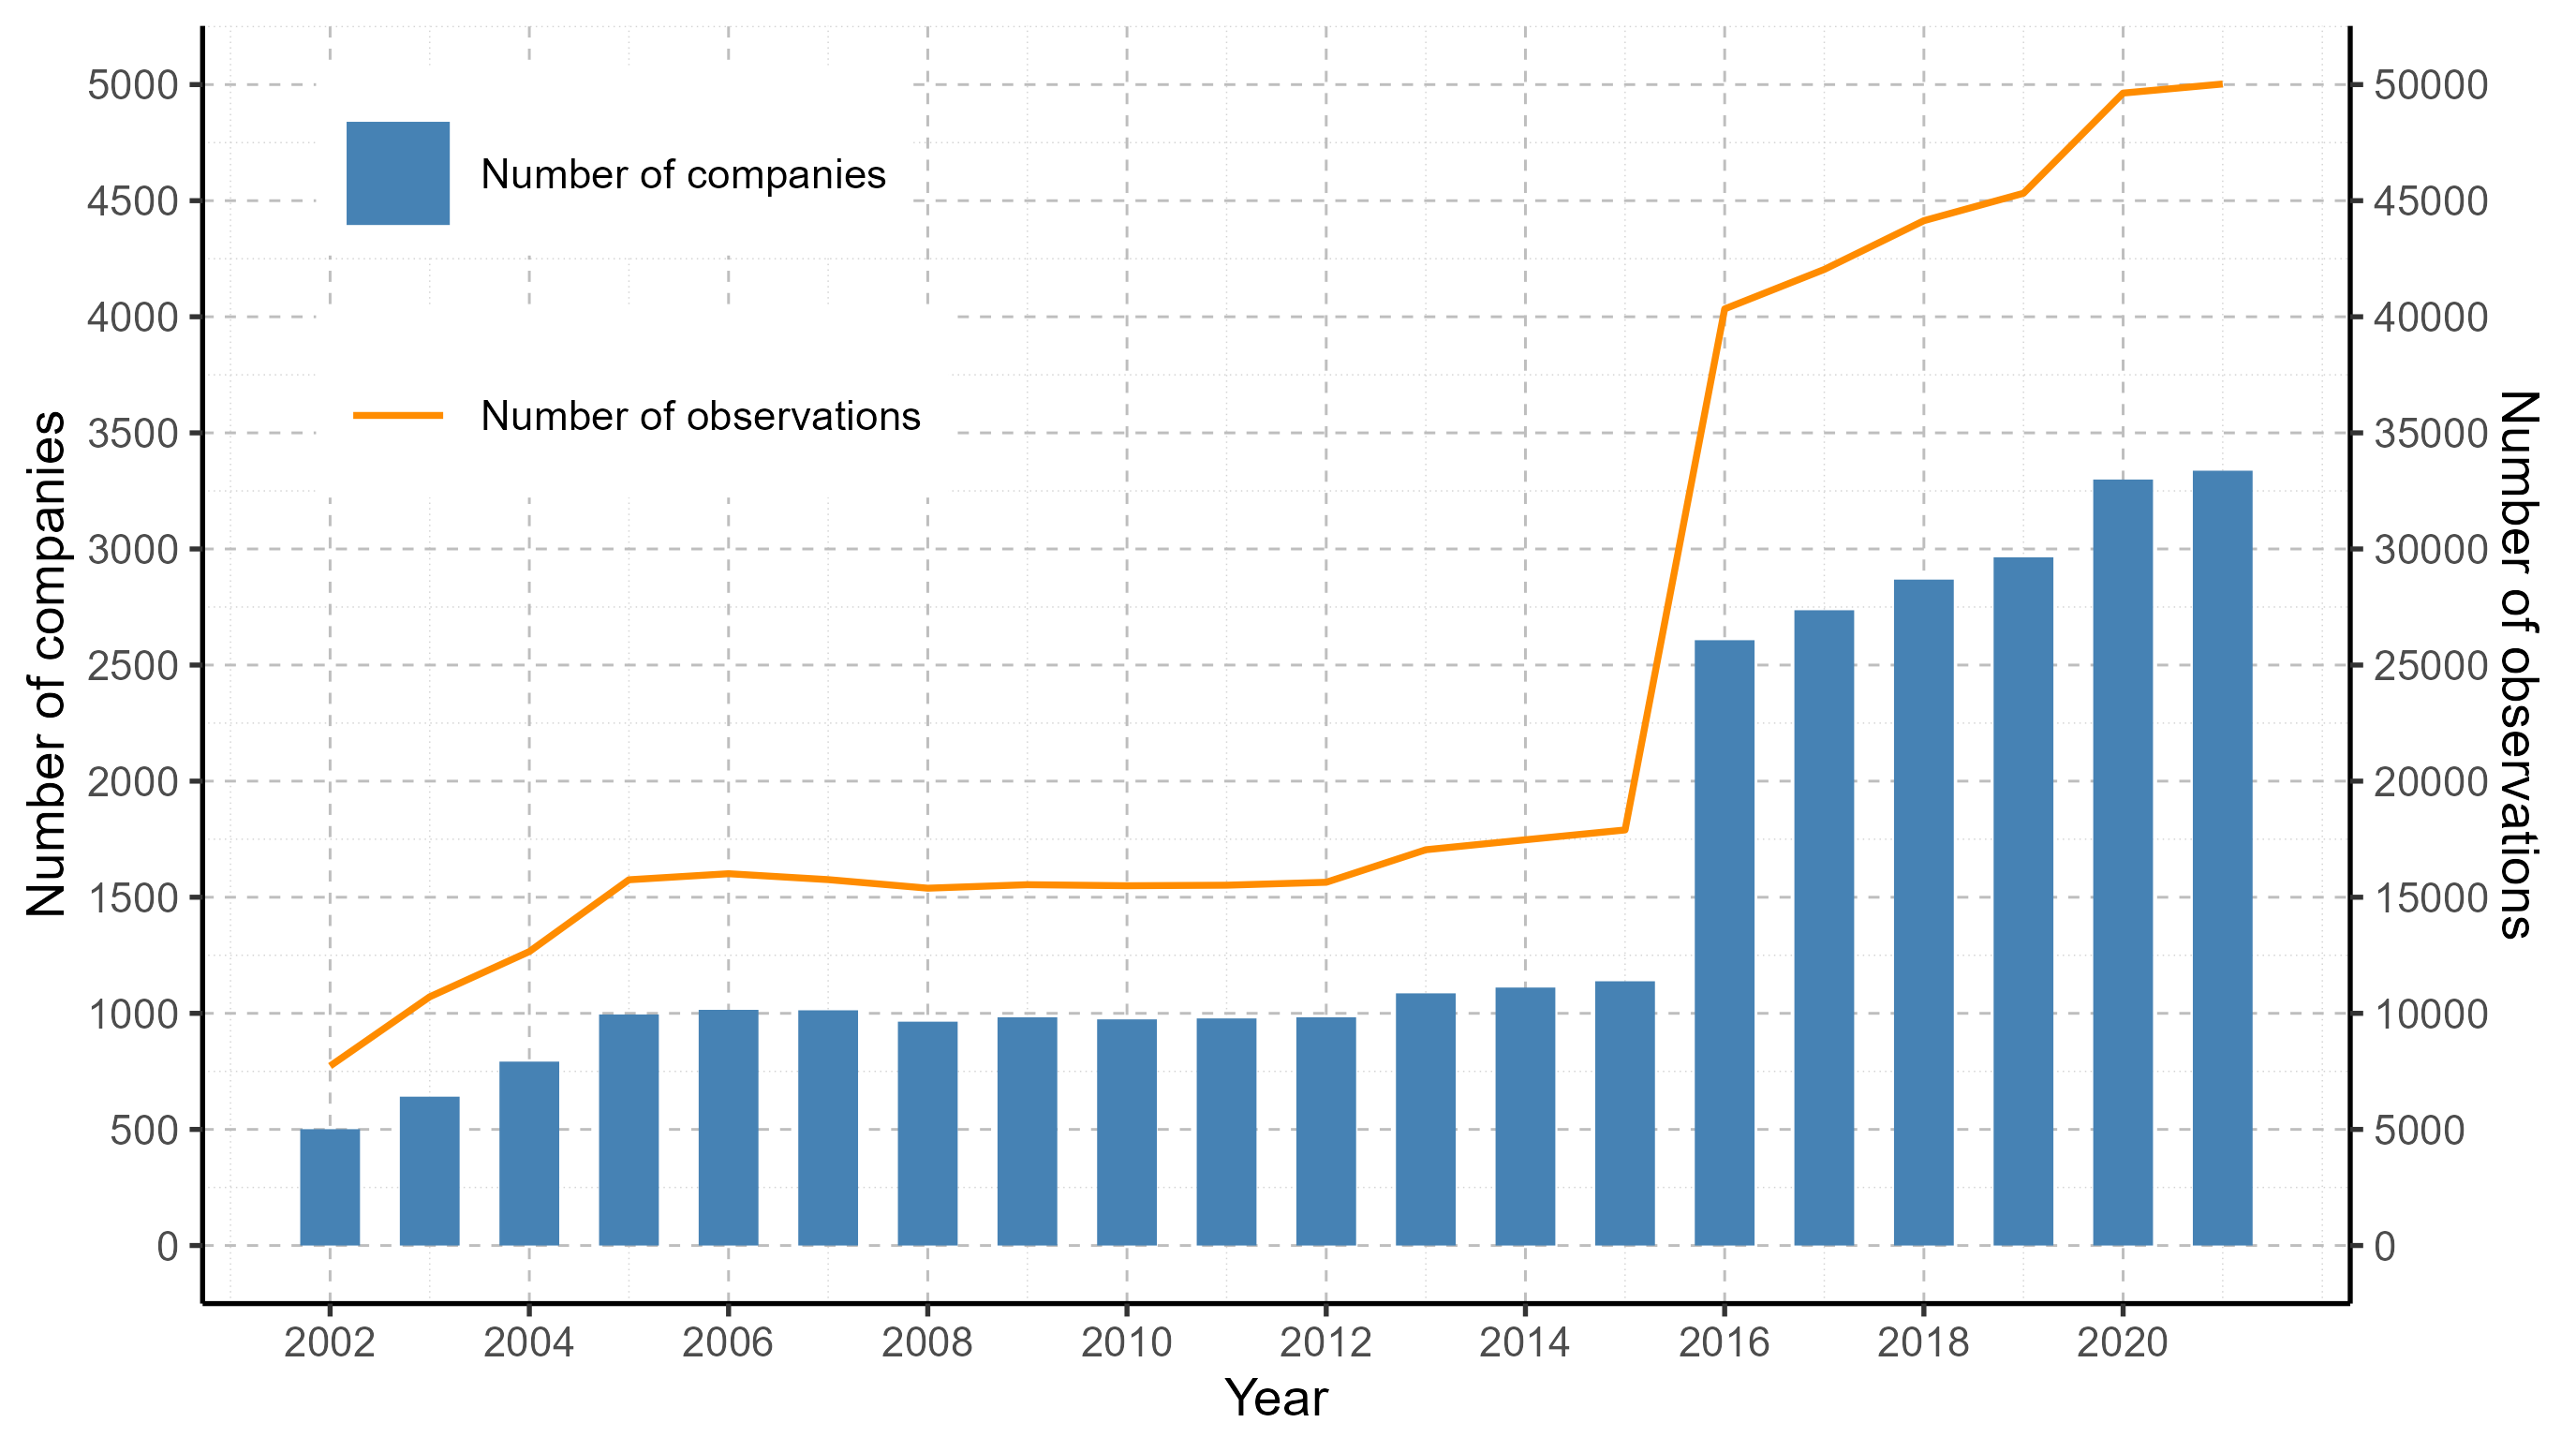
\includegraphics{image/number_p.png}
\label{fig: num}
\caption*{\footnotesize{This graphic plots the number of firms and observations across the whole sample period.}}
\end{figure}

%%%%%%%%%%%%%%%%%%%%%%%%%%%%%%%%%%%%%%%%%%%%%%%%%%%
\subsection{Variable definition and summary statistics}

We provide concise explanations for key variables outlined in Table \ref{tab: var def}. The stock return data incorporates stocks' capital gains and dividends, observed monthly. The companies' total carbon emission data is the sum of all 3 scopes of emissions: Scope 1 entails direct greenhouse gas emissions, Scope 2 covers indirect emissions from purchased energy consumption, and Scope 3 encompasses a wider range of upstream and downstream indirect emissions. While, carbon intensity is calculated as the ratio of carbon emissions to revenue, indicating how effectively a company utilizes its CO2 emissions to generate revenue. Control variables in this analysis encapsulate fundamental financial conditions, which have been substantiated as pertinent factors influencing stock returns through extensive literature such as \cite{aswani2023carbon}, \cite{bolton2023carbon}, and \cite{oestreich2015carbon}. The size is a firm's market capitalization in logarithmic form, serving as a measure of its size; leverage, which quantifies a firm's financial risk by assessing the ratio of total liability to market capitalization; B/M (Book-to-Market Ratio) indicating the difference between firms' book value and market valuation; RoE (Return on Equity) capturing firms' profitability through the return generated on shareholders' equity; Invest/AT (Investment to Total Assets) reflecting firms' innovation efforts by scaling investment with total assets; PPE (Property, Plant, and Equipment) measuring their fixed assets; SaleGR (Sales Growth) gauging revenue growth; EPS (Earnings Per Share) as another indicator of profitability; Staff\_num, the number of employees presented in logarithmic form; and Firm\_age, representing the firm's age since its foundation. These variables collectively provide insights into various financial, operational, and growth aspects that are pertinent to our analysis of the interplay between environmental factors and stock returns.

\begin{table}[!ht]
\footnotesize
\centering
\caption{\textbf{Variable Definition}}
\label{tab: var def}
\begin{tabular}{ll}
\toprule
Variables & Definition \\ \hline

\textit{RET} & Monthly stock return \\
\textit{Co2\_tot} & Total carbon emissions (log) \\
\textit{Co2\_int} & Carbon intensity \\
\textit{Size} & Total market capitalization (log) \\
\textit{Leverage} & Total liability over market capitalization \\
\textit{B/M} & Book to market ratio \\
\textit{RoE} & Return on equity \\
\textit{Inves/AT} & Investment over total assets \\
\textit{PPE} & Property, plant, and equipment (log) \\
\textit{SaleGR} & Growth in revenue \\
\textit{EPS} & Earning per share \\
\textit{Staff\_num} & Number of employees (log) \\
\textit{Firm\_age} & Firm age since foundation\\
  
\bottomrule
\end{tabular}
\begin{tablenotes}
\footnotesize
\item This table presents the definition of variables used in our analysis.
\end{tablenotes}
\end{table}

%%%%%%%%%%%%%%%%%%%%%%%%%%%%%%%%%%%%%%%%%%%%%%%%%%%
Table \ref{tab: summ stats} provides a summary of the statistical characteristics for the majority of variables used in this study. To mitigate the potential impact of outliers, we have applied winsorization to some of the variables at various thresholds. This process involves capping extreme values to ensure that the dataset maintains a reasonable balance between standard deviation and mean values. Within the entire dataset, the monthly stock returns exhibit a range of -31.60\% to 40.10\%, with a mean value of 1.12\% following the winsorization procedure at 1\% level. Firms' total CO2 emissions, on the other hand, span a range from 0.27 to 41.44 million tons per year. After log normalization, the standard deviation of CO2 emissions stands at 2.76, reflecting variations in emissions levels across the sample. B/M (Book to market ratio, SaleGR (Growth in avenue), and EPS (Earning per share) are all winsorized at 1\% level. 

\begin{table}[!ht]
\centering
\footnotesize
\caption{\textbf{Summary Statistics}}
\label{tab: summ stats}
\begin{tabular}{lcrrrrrr}
\toprule
{} &  Winsorized Level &    count &   mean &   std &     min &    50\% &    max \\
\midrule
RET      & 1\%    & 466999 &  1.116 & 9.913 & -31.596 &  1.023 & 40.095 \\
Co2\_tot   &  -  & 480119 & 12.643 & 2.764 &   0.237 & 12.853 & 19.842 \\
Intensity\_tot &  - & 480119 &  4.994 & 1.321 &   3.065 &  4.859 & 11.407 \\
Size     &  -   & 416091 &  8.300 & 1.869 &   0.008 &  8.291 & 20.722 \\
Levarage  &  -  & 479175 &  0.641 & 0.269 &   0.001 &  0.644 &  6.925 \\
B/M       &  1\%  & 406753 &  0.529 & 0.429 &  -0.384 &  0.432 &  2.972 \\
RoE       &  -  & 409460 &  0.066 & 0.397 &  -3.324 &  0.105 &  2.590 \\
Inves/AT  &  -  & 416447 &  0.042 & 0.052 &  -0.186 &  0.026 &  0.869 \\
PPE       &  -  & 402241 &  7.040 & 2.542 &   0.000 &  7.240 & 13.362 \\
SaleGR    &  1\%  & 420518 &  0.103 & 0.275 &  -0.591 &  0.063 &  2.423 \\
EPS       &  1\%  & 410364 &  1.918 & 3.146 &  -9.400 &  1.580 & 19.820 \\
Staff\_num  & -  & 472193 &  2.212 & 1.519 &   0.000 &  2.100 &  7.741 \\
Firm\_age   & -  & 472563 &  4.078 & 0.799 &   1.099 &  4.127 &  6.489 \\
\bottomrule

\end{tabular}
\begin{tablenotes}
    \item The table reports the sample means of the main variables over the whole sample period. All variables are defined in Table \ref{tab: var def}.
\end{tablenotes}
\end{table}

%%%%%%%%%%%%%%%%%%%%%%%%%%%%%%%%%%%%%%%%%%%%%%%%%%%
In Table \ref{tab: corr}, we report the pairwise Pearson correlations among all the control variables. Notably, two carbon footprint indicators, namely total carbon emissions and emission intensity, exhibit a positive correlation. However, the correlation coefficient of 0.63 suggests some divergence between these two indicators. Firms' size demonstrates a strong positive correlation with their total CO2 emissions, with a coefficient of 0.68. This implies that larger firms tend to have higher total CO2 emissions. Conversely, the correlation between firm size and CO2 intensity is only 0.09, indicating a lack of a strong relationship between firm size and its carbon intensity. This highlights that larger firms may have varying levels of carbon intensity, with some large firms exhibiting low carbon intensity. The highest correlations are observed between PPE (Property, Plant, and Equipment) and CO2 emissions, PPE and firm size, Staff\_num (number of employees) and total CO2 emissions, and Staff\_num and firm size. In each of these cases, the correlation exceeds 0.7 in absolute value, signifying that firms with more PPE and a greater number of employees tend to be larger firms with higher CO2 emissions. Nevertheless, these correlations do not indicate a strong association with CO2 intensity, emphasizing that the relationship between firm characteristics and carbon intensity is not as pronounced.

\begin{landscape}
\begin{table}[!ht]
\scriptsize
\centering
\def\sym#1{\ifmmode^{#1}\else\(^{#1}\)\fi}
\caption{\textbf{Control Variables' Pearson Correlation}}
\label{tab: corr}
\begin{tabular}{lllllllllllll}
\toprule
 & Co2\_tot & Intensity\_tot & Size & Levarage & B/M & RoE & Inves/AT & PPE & SaleGR & EPS & Staff\_num & Firm\_age \\
 \hline
Co2\_tot & 1.0*** & 0.63*** & 0.68*** & -0.0 & 0.02*** & 0.24*** & 0.25*** & 0.84*** & -0.09*** & 0.3*** & 0.74*** & 0.31*** \\
Intensity\_tot &  & 1.0*** & 0.09*** & -0.26*** & -0.01*** & 0.02*** & 0.37*** & 0.45*** & -0.03*** & -0.01*** & 0.15*** & 0.01*** \\
Size &  &  & 1.0*** & 0.05*** & -0.21*** & 0.24*** & 0.06*** & 0.71*** & 0.01** & 0.38*** & 0.73*** & 0.3*** \\
Levarage &  &  &  & 1.0*** & -0.02*** & 0.06*** & -0.11*** & 0.14*** & -0.09*** & 0.05*** & 0.12*** & 0.24*** \\
B/M &  &  &  &  & 1.0*** & -0.08*** & -0.04*** & 0.12*** & -0.12*** & -0.07*** & -0.04*** & 0.05*** \\
RoE &  &  &  &  &  & 1.0*** & 0.03*** & 0.2*** & 0.03*** & 0.39*** & 0.2*** & 0.19*** \\
Inves/AT &  &  &  &  &  &  & 1.0*** & 0.32*** & 0.06*** & 0.01*** & 0.05*** & -0.05*** \\
PPE &  &  &  &  &  &  &  & 1.0*** & -0.11*** & 0.28*** & 0.71*** & 0.36*** \\
SaleGR &  &  &  &  &  &  &  &  & 1.0*** & 0.05*** & -0.12*** & -0.17*** \\
EPS &  &  &  &  &  &  &  &  &  & 1.0*** & 0.29*** & 0.24*** \\
Staff\_num &  &  &  &  &  &  &  &  &  &  & 1.0*** & 0.36*** \\
Firm\_age &  &  &  &  &  &  &  &  &  &  &  & 1.0*** \\
\bottomrule
\multicolumn{7}{l}{\footnotesize * p\sym{<}.1, ** p\sym{<}.05, *** p\sym{<}.01}
\end{tabular}
\begin{tablenotes}
    \item This table reports the pairwise Pearson correlations among all the control variables and firms' carbon footprint variables. * means significance at 10\%, ** at 5\%, *** at 1\%.
\end{tablenotes}
\end{table}
\end{landscape}

%%%%%%%%%%%%%%%%%%%%%%%%%%%%%%%%%%%%%%%%%%%%%%%%%%%
\subsection{CO2 Emissions \& CO2 Intensity}

In the current corporate finance literature there are two important indicators quantifying firms' carbon footprints. Alongside firms' total CO2 emissions, CO2 intensity emerges as a critical metric for evaluating their environmental sustainability. CO2 intensity precisely measures the rate of emissions of a specific pollutant concerning the scale of firms' production activities. In our study, we employ CO2 intensity, calculated as firms' total CO2 emissions normalized by their revenue, as a means to assess their emission efficiency.

Figure \ref{fig: co2_intensity} illustrates the historical trajectory of firms' carbon footprints, as represented by both their total CO2 emissions and CO2 intensity. Across the entire sampling period, we observe a consistent downward trend in both metrics for measuring firms' carbon footprint. Notably, a substantial decline is evident in the year 2016 for both total CO2 emissions and intensity. This reduction can primarily be attributed to the expanded data coverage of the TRUCOST database in that year, encompassing a broader spectrum of small and medium-sized companies. The overarching decline in both CO2 emissions and intensity, except for the significant drop in 2016, underscores the collective endeavor towards greener practices by companies. Furthermore, it reflects the tangible impact of effective green policies on shaping firms' environmental behavior and fostering environmentally conscious practices.

\begin{figure}[!ht]
\centering
\caption{\textbf{CO2 Emissions \& CO2 Intensity}}
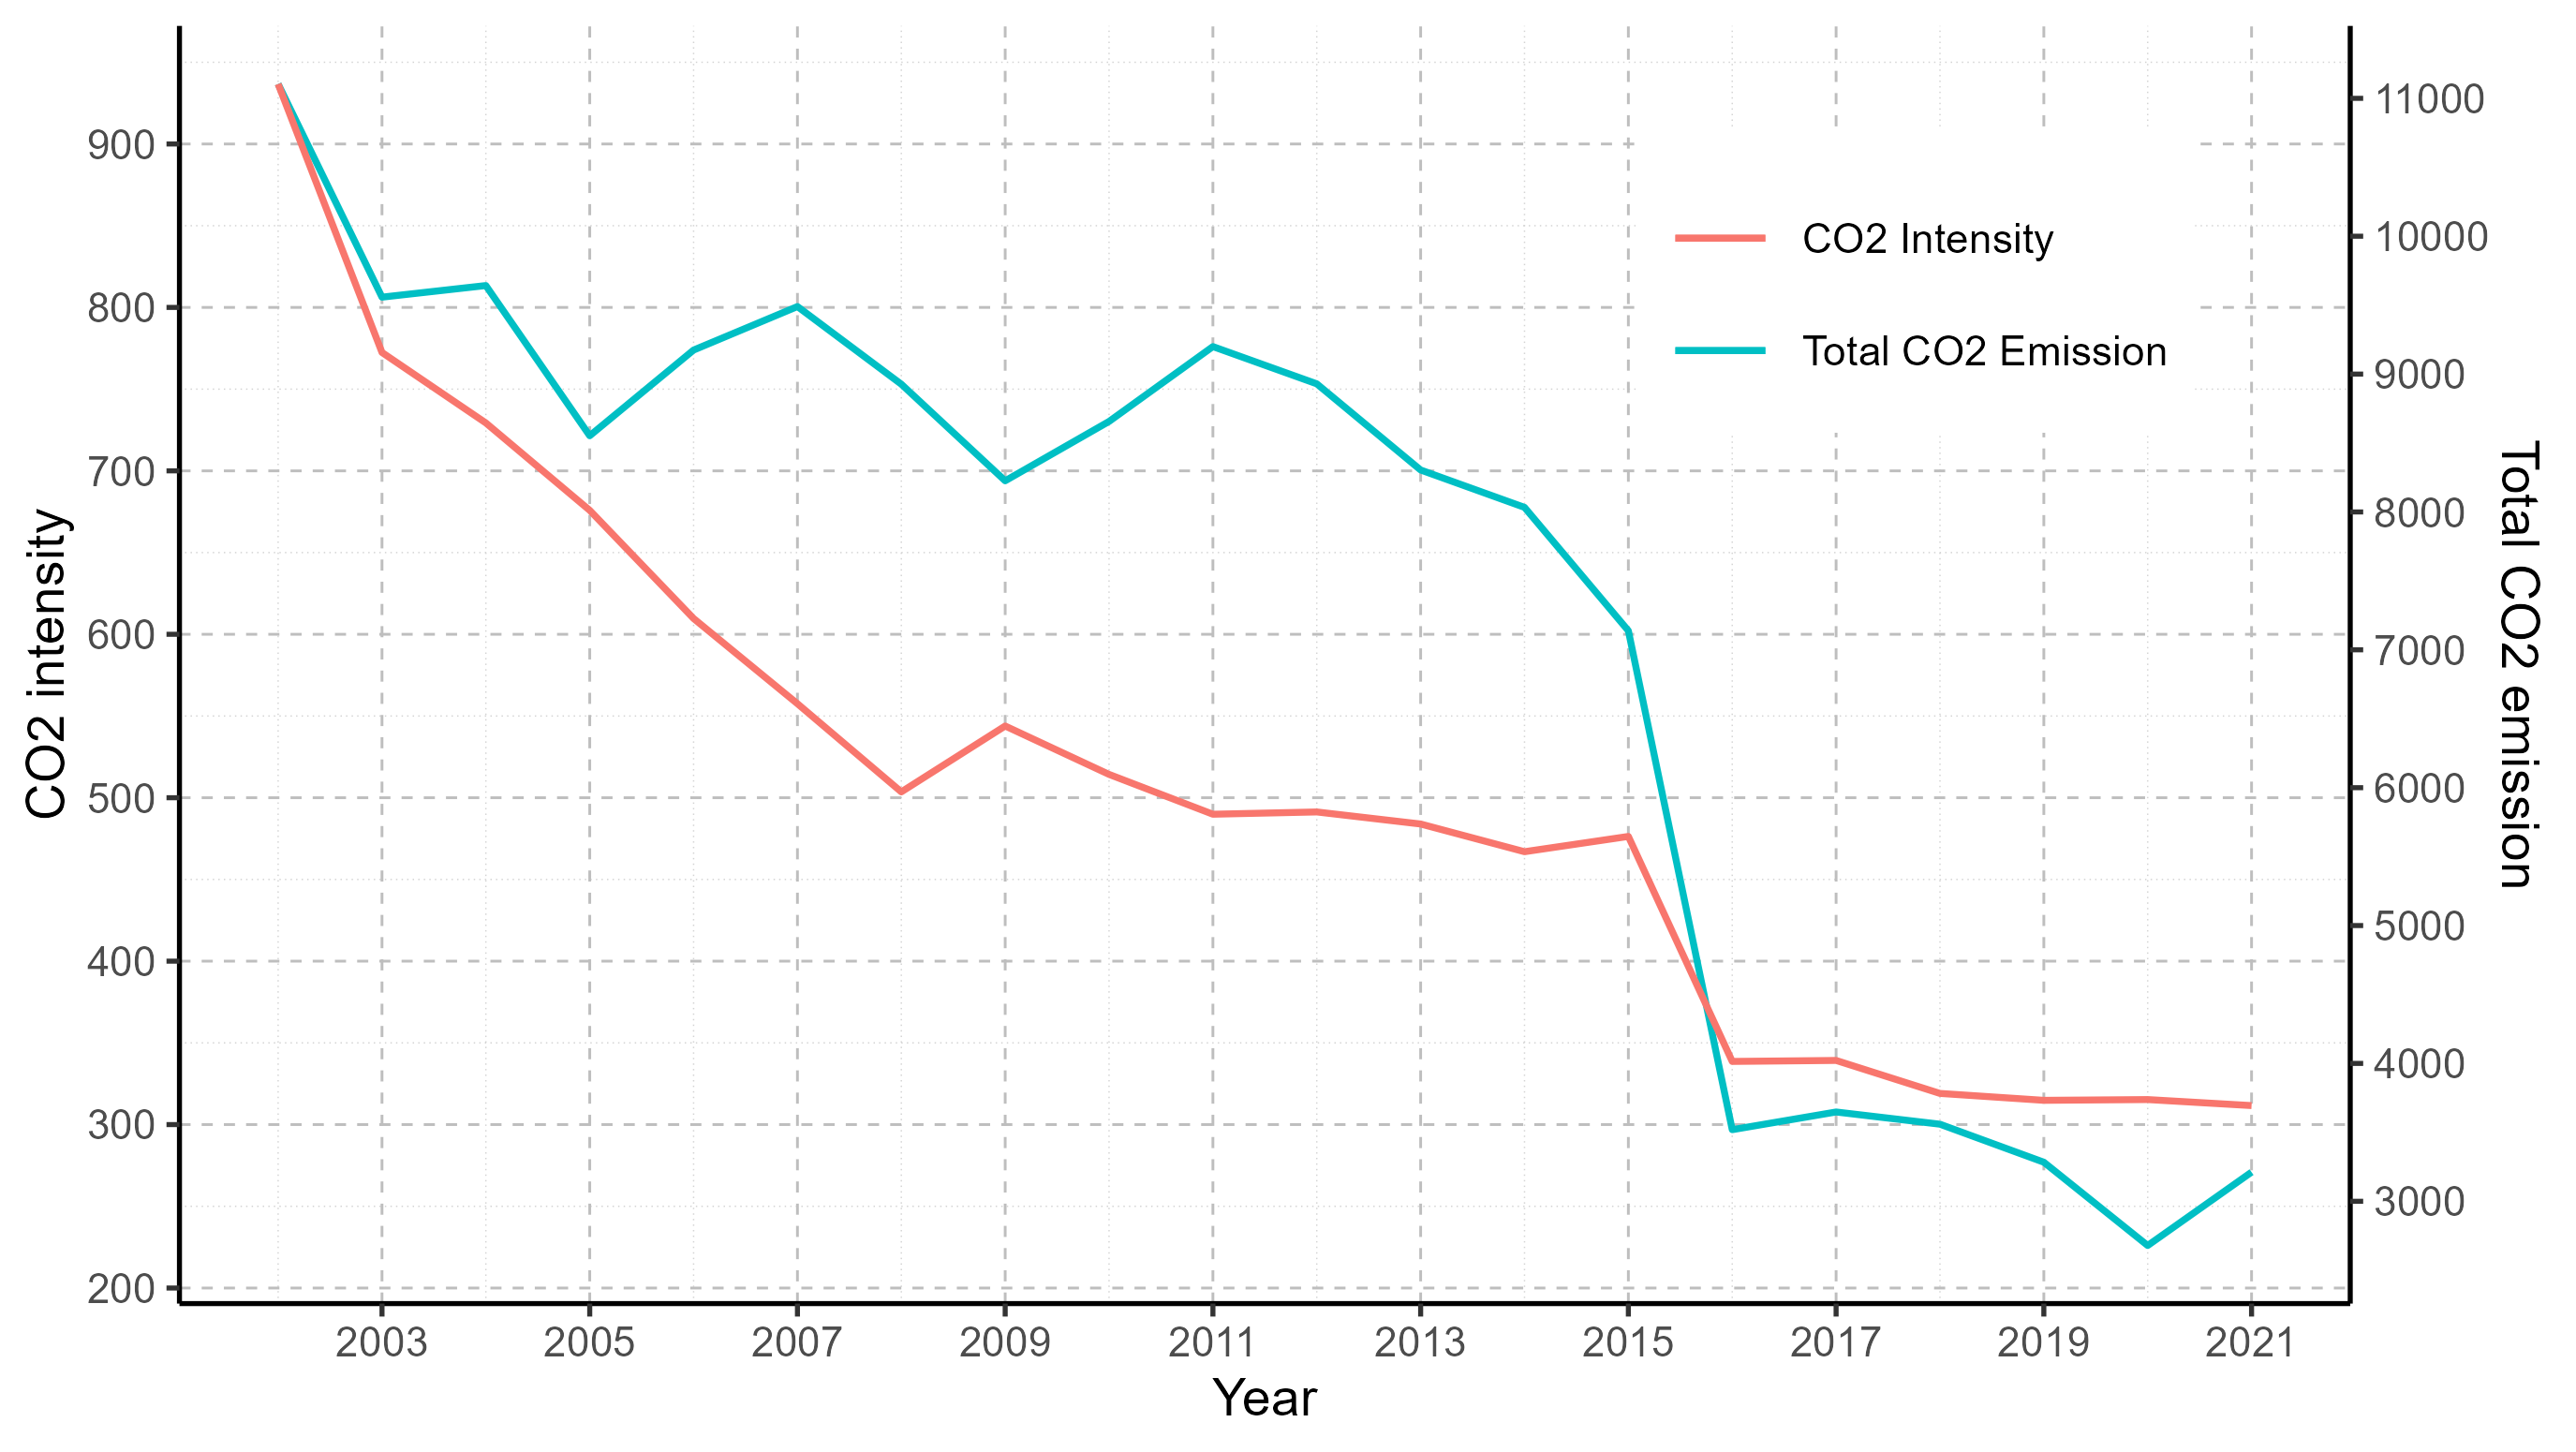
\includegraphics{image/co2_total_p.png}
\label{fig: co2_intensity}
\caption*{\footnotesize{This graphic illustrates the historical trajectory of firms' total CO2 emissions and intensity. Firms' total CO2 emissions are measured in thousand tons, while intensity is quantified by tons of CO2 emitted per million US dollars of revenue.}}
\end{figure}

%%%%%%%%%%%%%%%%%%%%%%%%%%%%%%%%%%%%%%%%%%%%%%%%%%%
\subsection{Total CO2 Emissions in Different Industries}

Table \ref{tab: industries rank} provides a ranking of industries according to their average total CO2 emissions over the period from 2002 to 2021. Notably, the industries with the most substantial average CO2 emissions are Independent Power and Renewable Electricity Productions, which exhibit an annual average of approximately 47.15 million tons. Electric Utilities and Oil, Gas, and Consumable Fuels secure the second and third positions, emitting around 40.93 million and 35.12 million tons of CO2 on average during the entire sampling period, respectively. These sectors are renowned for their notable environmental impacts due to the higher levels of CO2 emissions they generate. On the contrary, industries with the least average CO2 emissions encompass Transportation Infrastructure, Mortgage Real Estate Investment Trusts (REITs), and Health Care Technology, showcasing relatively smaller environmental footprints based on their total CO2 emissions.

Taking into account the entire sampling period and a comprehensive range of industries, the average greenhouse gas emissions stand at 4.64 million tons. Strikingly, the most environmentally impactful sector, exemplified by Independent Power and Renewable Electricity Productions, demonstrates total CO2 emissions that are nearly ten times higher than the average. In contrast, the most environmentally friendly industry, like Health Care Technology, emits only approximately 1/100th of the average emissions. This highlights a substantial diversity across industries concerning their total carbon emissions, underlining the significant heterogeneity in their environmental impacts.

%%%%%%%%%%%%%%%%%%%%%%%%%%%%%%%%%%%%%%%%%%%%%%%%%%
\begin{landscape}
\begin{table}[!ht]
\scriptsize
\centering
\caption{Industries Ranked by Average Total CO2 Emission}
\label{tab: industries rank}
\begin{tabular}{clcclc}
\toprule
 Rank &                                 GICS Industry Name &  Total CO2 Emission &  Rank &                               GICS Industry Name &  Total CO2 Emission \\
\midrule
   1 & Power and Renewable Elec... &               47.15 &    34 &                                    Gas Utilities &                1.89 \\
    2 &                                 Electric Utilities &               40.93 &    35 &                             Electrical Equipment &                1.54 \\
    3 &                      Oil, Gas and Consumable Fuels &               35.12 &    36 &                  Hotels, Restaurants and Leisure &                1.45 \\
    4 &                                        Automobiles &               30.26 &    37 &       Semiconductors and Semiconductor Equipment &                1.37 \\
    5 &                                    Multi-Utilities &               22.74 &    38 &                 Commercial Services and Supplies &                1.35 \\
    6 &                                 Passenger Airlines &               16.42 &    39 & Electronic Equipment, Instruments and Components &                1.33 \\
    7 &                           Industrial Conglomerates &               15.41 &    40 &               Textiles, Apparel and Luxury Goods &                1.19 \\
    8 &                                 Financial Services &               14.98 &    41 &                     Construction and Engineering &                1.11 \\
    9 &                                  Metals and Mining &               14.76 &    42 &                         Communications Equipment &                1.10 \\
   10 &                             Construction Materials &               13.60 &    43 &               Health Care Equipment and Supplies &                1.06 \\
   11 &                                      Food Products &               12.99 &    44 &                                 Specialty Retail &                1.05 \\
   12 &                                          Chemicals &               10.13 &    45 &                            Marine Transportation &                1.04 \\
   13 &                             Personal Care Products &                9.61 &    46 &               Trading Companies and Distributors &                0.95 \\
   14 &                                            Tobacco &                8.48 &    47 &                   Interactive Media and Services &                0.94 \\
   15 &           Consumer Staples Distribution and Retail &                8.42 &    48 &                                      IT Services &                0.93 \\
   16 &                                 Household Products &                7.69 &    49 &                                 Leisure Products &                0.86 \\
   17 &                              Aerospace and Defense &                7.41 &    50 &                 Life Sciences Tools and Services &                0.70 \\
   18 &                          Air Freight and Logistics &                7.05 &    51 &                                     Distributors &                0.63 \\
   19 &                           Containers and Packaging &                6.56 &    52 &                                  Capital Markets &                0.60 \\
   20 &                                          Beverages &                6.18 &    53 &                                            Media &                0.59 \\
   21 &                          Paper and Forest Products &                5.05 &    54 &                                    Entertainment &                0.53 \\
   22 &       Technology Hardware, Storage and Peripherals &                4.18 &    55 &                                        Insurance &                0.42 \\
   23 &                              Automobile Components &                3.85 &    56 &                                  Water Utilities &                0.33 \\
   24 &                                  Building Products &                2.98 &    57 &                                            Banks &                0.27 \\
   25 &                              Ground Transportation &                2.95 &    58 &                                         Software &                0.27 \\
   26 &                                 Household Durables &                2.82 &    59 &                    Diversified Consumer Services &                0.26 \\
   27 &             Diversified Telecommunication Services &                2.52 &    60 &                                 Consumer Finance &                0.25 \\
   28 &                                          Machinery &                2.46 &    61 &                            Professional Services &                0.24 \\
   29 &                 Health Care Providers and Services &                2.42 &    62 &           Real Estate Management and Development &                0.20 \\
   30 &                      Energy Equipment and Services &                2.27 &    63 &                                    Biotechnology &                0.12 \\
   31 &                                    Pharmaceuticals &                2.20 &    64 &                    Transportation Infrastructure &                0.07 \\
   32 &                Wireless Telecommunication Services &                1.94 &    65 &   Mortgage Real Estate Investment Trusts (REITs) &                0.04 \\
   33 &                                   Broadline Retail &                1.93 &    66 &                           Health Care Technology &                0.03 \\
\bottomrule
\end{tabular}
\begin{tablenotes}
\footnotesize
\item This table presents the ranking of different industries based on their average total CO2 emissions. The measurements for total CO2 emissions are provided in million tons. And the industry is categorized according to the GICS (Global Industry Classification Standard) industry classification.
\end{tablenotes}
\end{table}
\end{landscape}
\clearpage
%%%%%%%%%%%%%%%%%%%%%%%%%%%%%%%%%%%%%%%%%%%%%%%%%%%%%%%%%%%%%%%%
%%%%%%%%%%%%%%%%%%%%%%%%%%%%%%%%%%%%%%%%%%%%%%%%%%%%%%%%%%%%%%%%
\section{Result} \label{sec:result}
The main analysis of this paper tends to find the relationship between firms' carbon emissions and their stock returns. 
%%%%%%%%%%%%%%%%%%%%%%%%%%%%%%%%%%%%%%%%%%%%%%%%%%%
\subsection{Average Monthly Return on Firms' Carbon Footprint}

Our first practice delves into the unconditional relationship between firms' carbon footprint and their stock returns. Over the entire sample period, we adopt a cross-sectional approach, sorting CO2 emissions into 100 percentiles. Within each percentile, we compute the average monthly stock returns to gain an overarching understanding of the link between firms' CO2 emissions and their stock performance. Figure \ref{fig: co2_percentile} visually presents these findings. Panel A focuses on the average stock returns concerning firms' total CO2 emissions, while panels B, C, and D examine emissions within different scopes. Across all four panels, a distinguished downward trend emerges, indicating that firms with higher CO2 emissions tend to exhibit lower stock returns on average. Additionally, interesting patterns emerge. We observe peaks in average stock returns occurring when firms' CO2 emissions fall around the 1st percentile for all scopes. Another set of peaks in average returns is notable for different emissions categories, such as total CO2 emissions around the 55th percentile, scope 1 emissions near the 70th percentile, scope 2 emissions at approximately the 77th percentile, and scope 3 emissions around the 51st percentile. These clusters of companies may share common characteristics, possibly belonging to the same industry, with similarities in terms of size, profitability, and growth. It's important to note that in this analysis, we specifically sort firms based on their CO2 emissions only, without considering other stock return-related factors. Nevertheless, these initial findings provide valuable insights into the preliminary relationship between firms' CO2 emissions and their realized stock returns.

\begin{figure}[!ht]
\centering
\caption{\textbf{Average Stock Returns Based on CO2 Emissions}}
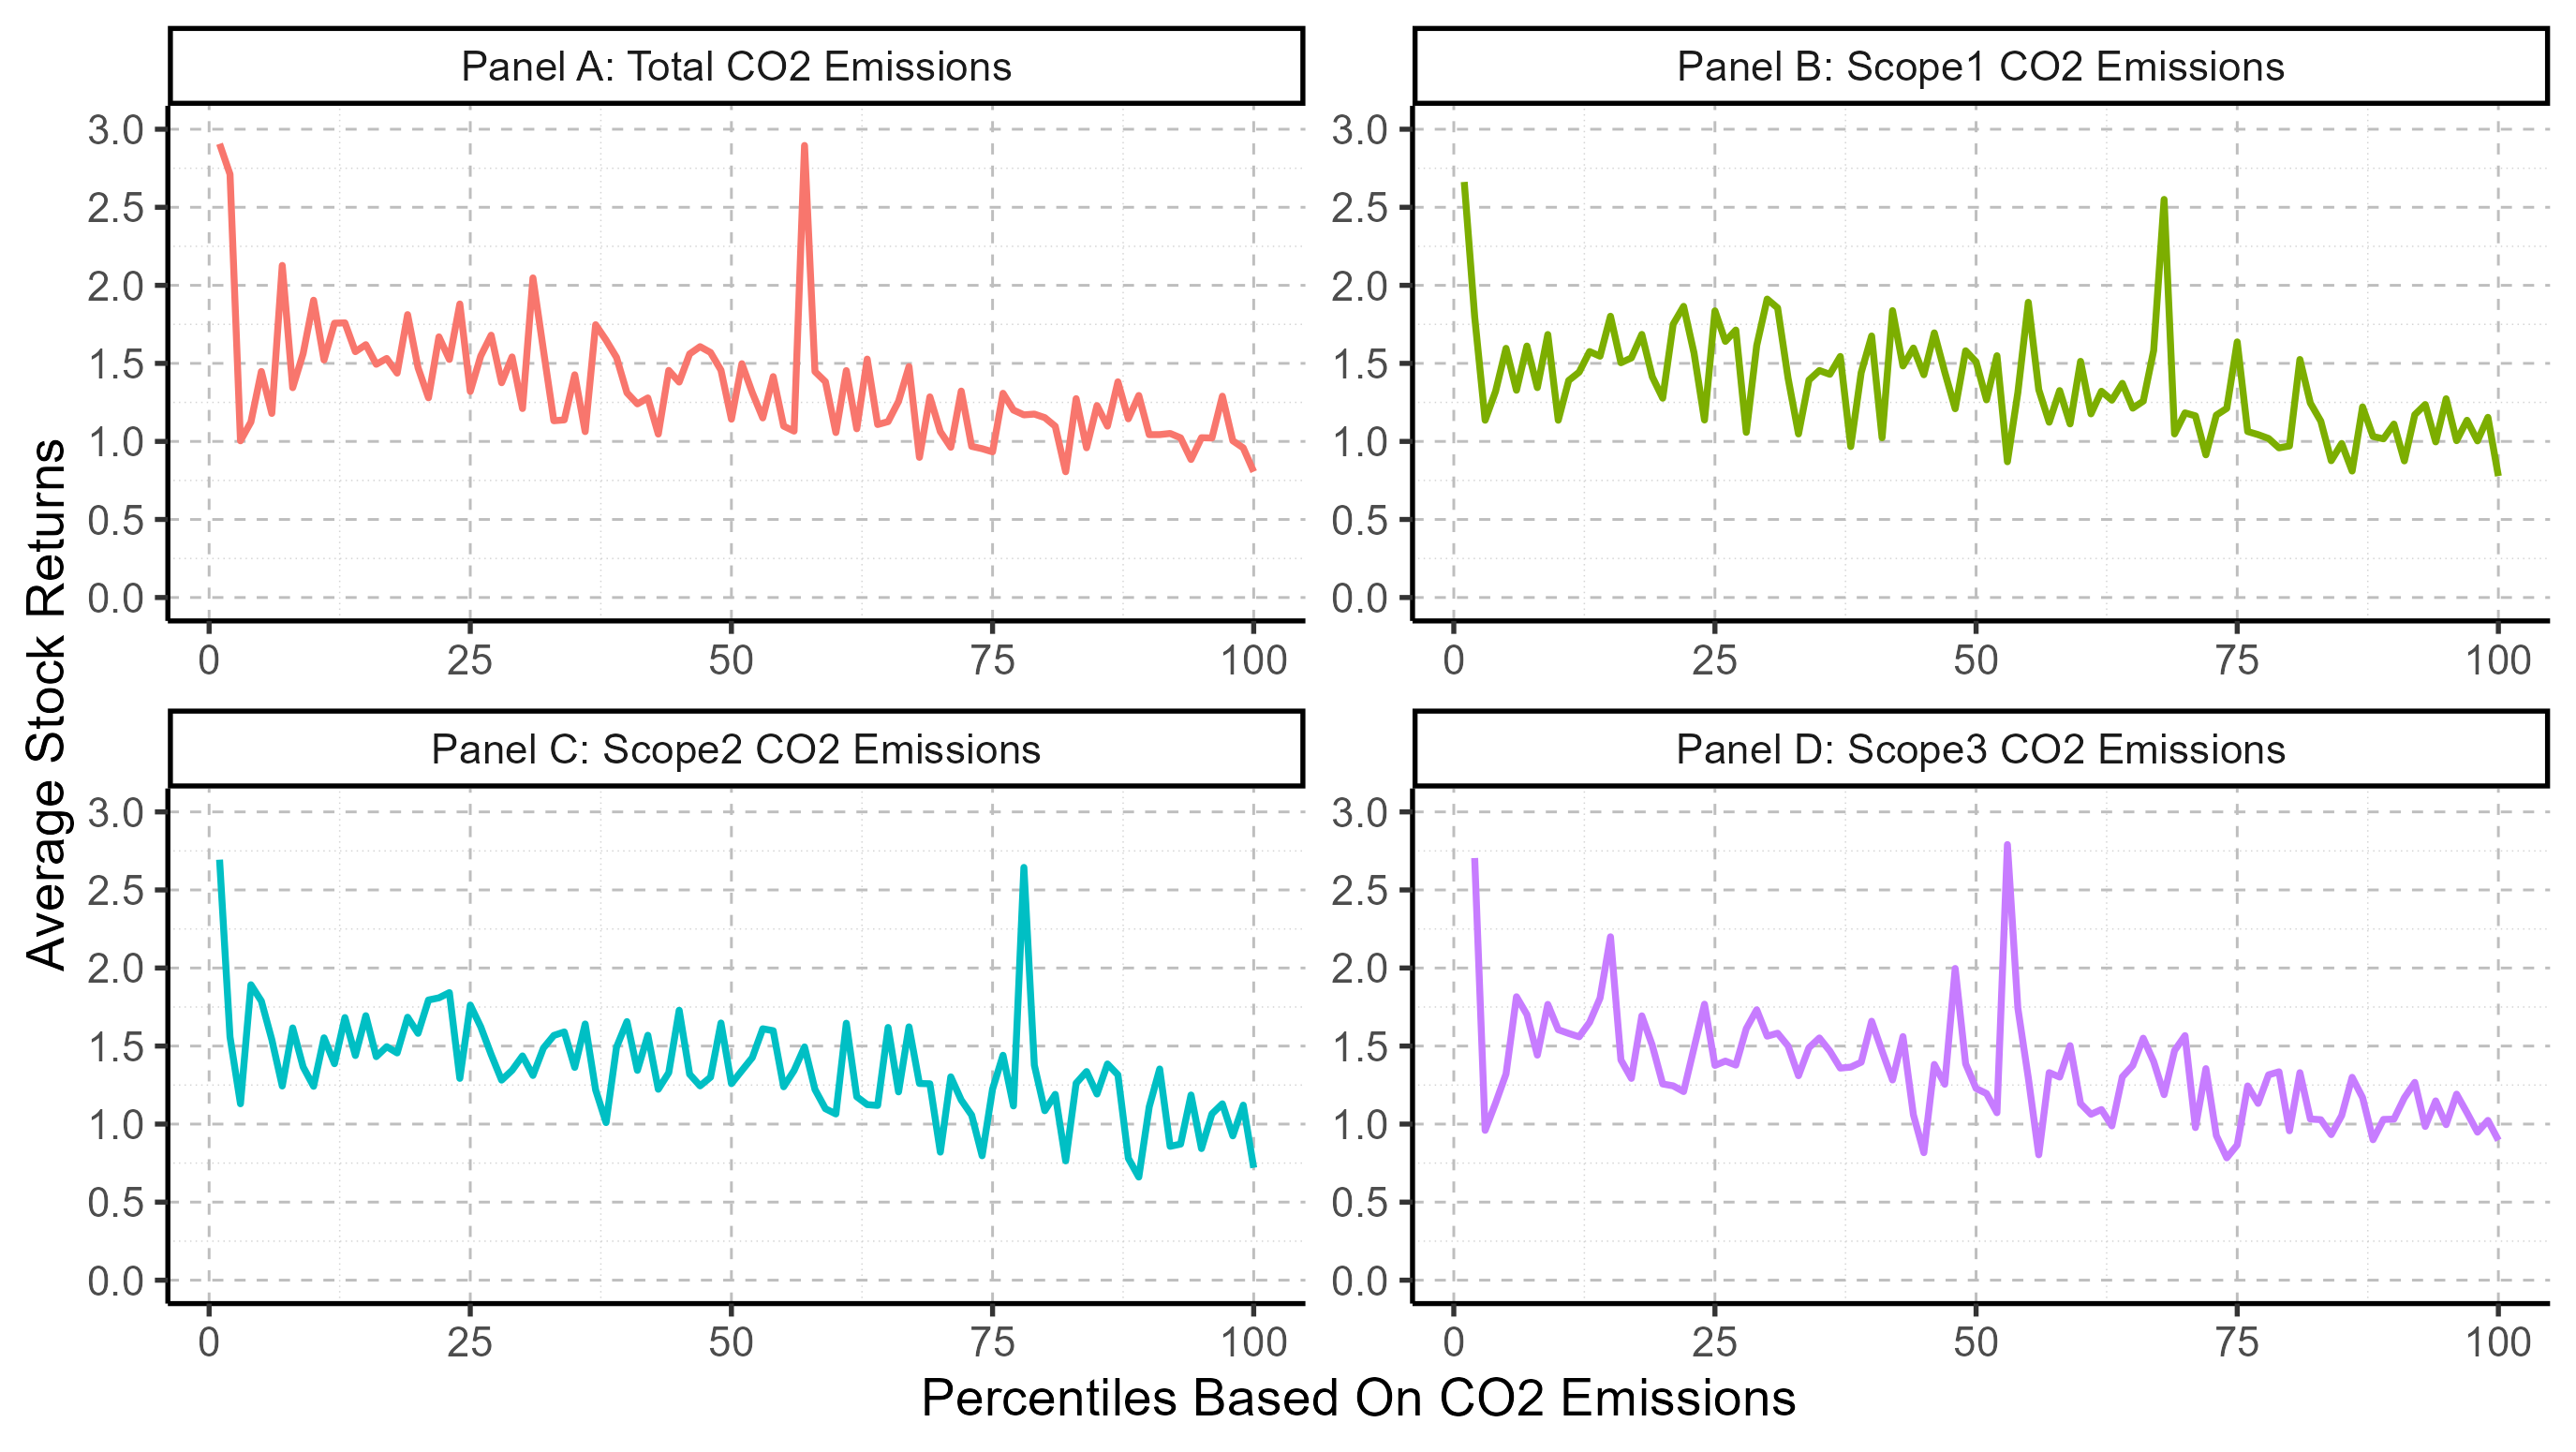
\includegraphics{image/co2_percentile.png}
\label{fig: co2_percentile}
\caption*{\footnotesize{This presents the average monthly stock returns in relation to different percentiles of CO2 emissions. Panel A depicts the average stock return in relation to firms' total CO2 emissions, while Panel B illustrates the average stock return concerning firms' scope 1 CO2 emissions. Panel C showcases the average stock return with respect to firms' scope 2 CO2 emissions, and Panel D presents the average stock return in connection with firms' scope 3 CO2 emissions.}}
\end{figure}

Following the same analytical approach, we explore whether a similar pattern emerges with another crucial indicator in corporate finance literature pertaining to firms' carbon footprint. Figure \ref{fig: intensity_percentile} illustrates the average monthly stock returns across different percentiles of firms' carbon intensity. In contrast to the previous analysis of CO2 emissions, we do not discern a clear and consistent trend in firms' average monthly stock returns across all four panels, where each representing different scopes of firms' carbon intensity. The absence of a discernible trend suggests that the relationship between firms' carbon intensity and their stock returns may not exhibit the same patterns as strongly as observed with CO2 emissions. 

Some may raise concerns that the robust relationship between firms' stock returns and CO2 emissions could be influenced by confounding factors such as firm size, leverage, profitability, and growth, as illustrated in Table \ref{tab: corr} the strong correlation between firms' CO2 emissions and some characteristic variables. Notably, the high and statistically significant positive correlation between firms' CO2 emissions and size. To address these concerns, we turn to Appendix Figure \ref{fig: others_persentile}, where we present the average monthly stock returns in relation to various firms' characteristics. In this analysis, we find that firms' size shows a positive association with stock returns within the first 25 percentiles. However, beyond this point, a clear relationship between these two indicators becomes less evident. While some patterns emerge in stock returns concerning variables like leverage, RoE (Return on Equity), and revenue growth, it's essential to note that these variables exhibit weak correlations with firms' CO2 emissions. This suggests that the observed relationship between CO2 emissions and stock returns remains robust, even after considering these potential confounding factors.

\begin{figure}[!ht]
\centering
\caption{\textbf{Average Stock Returns Based on CO2 Intensity}}
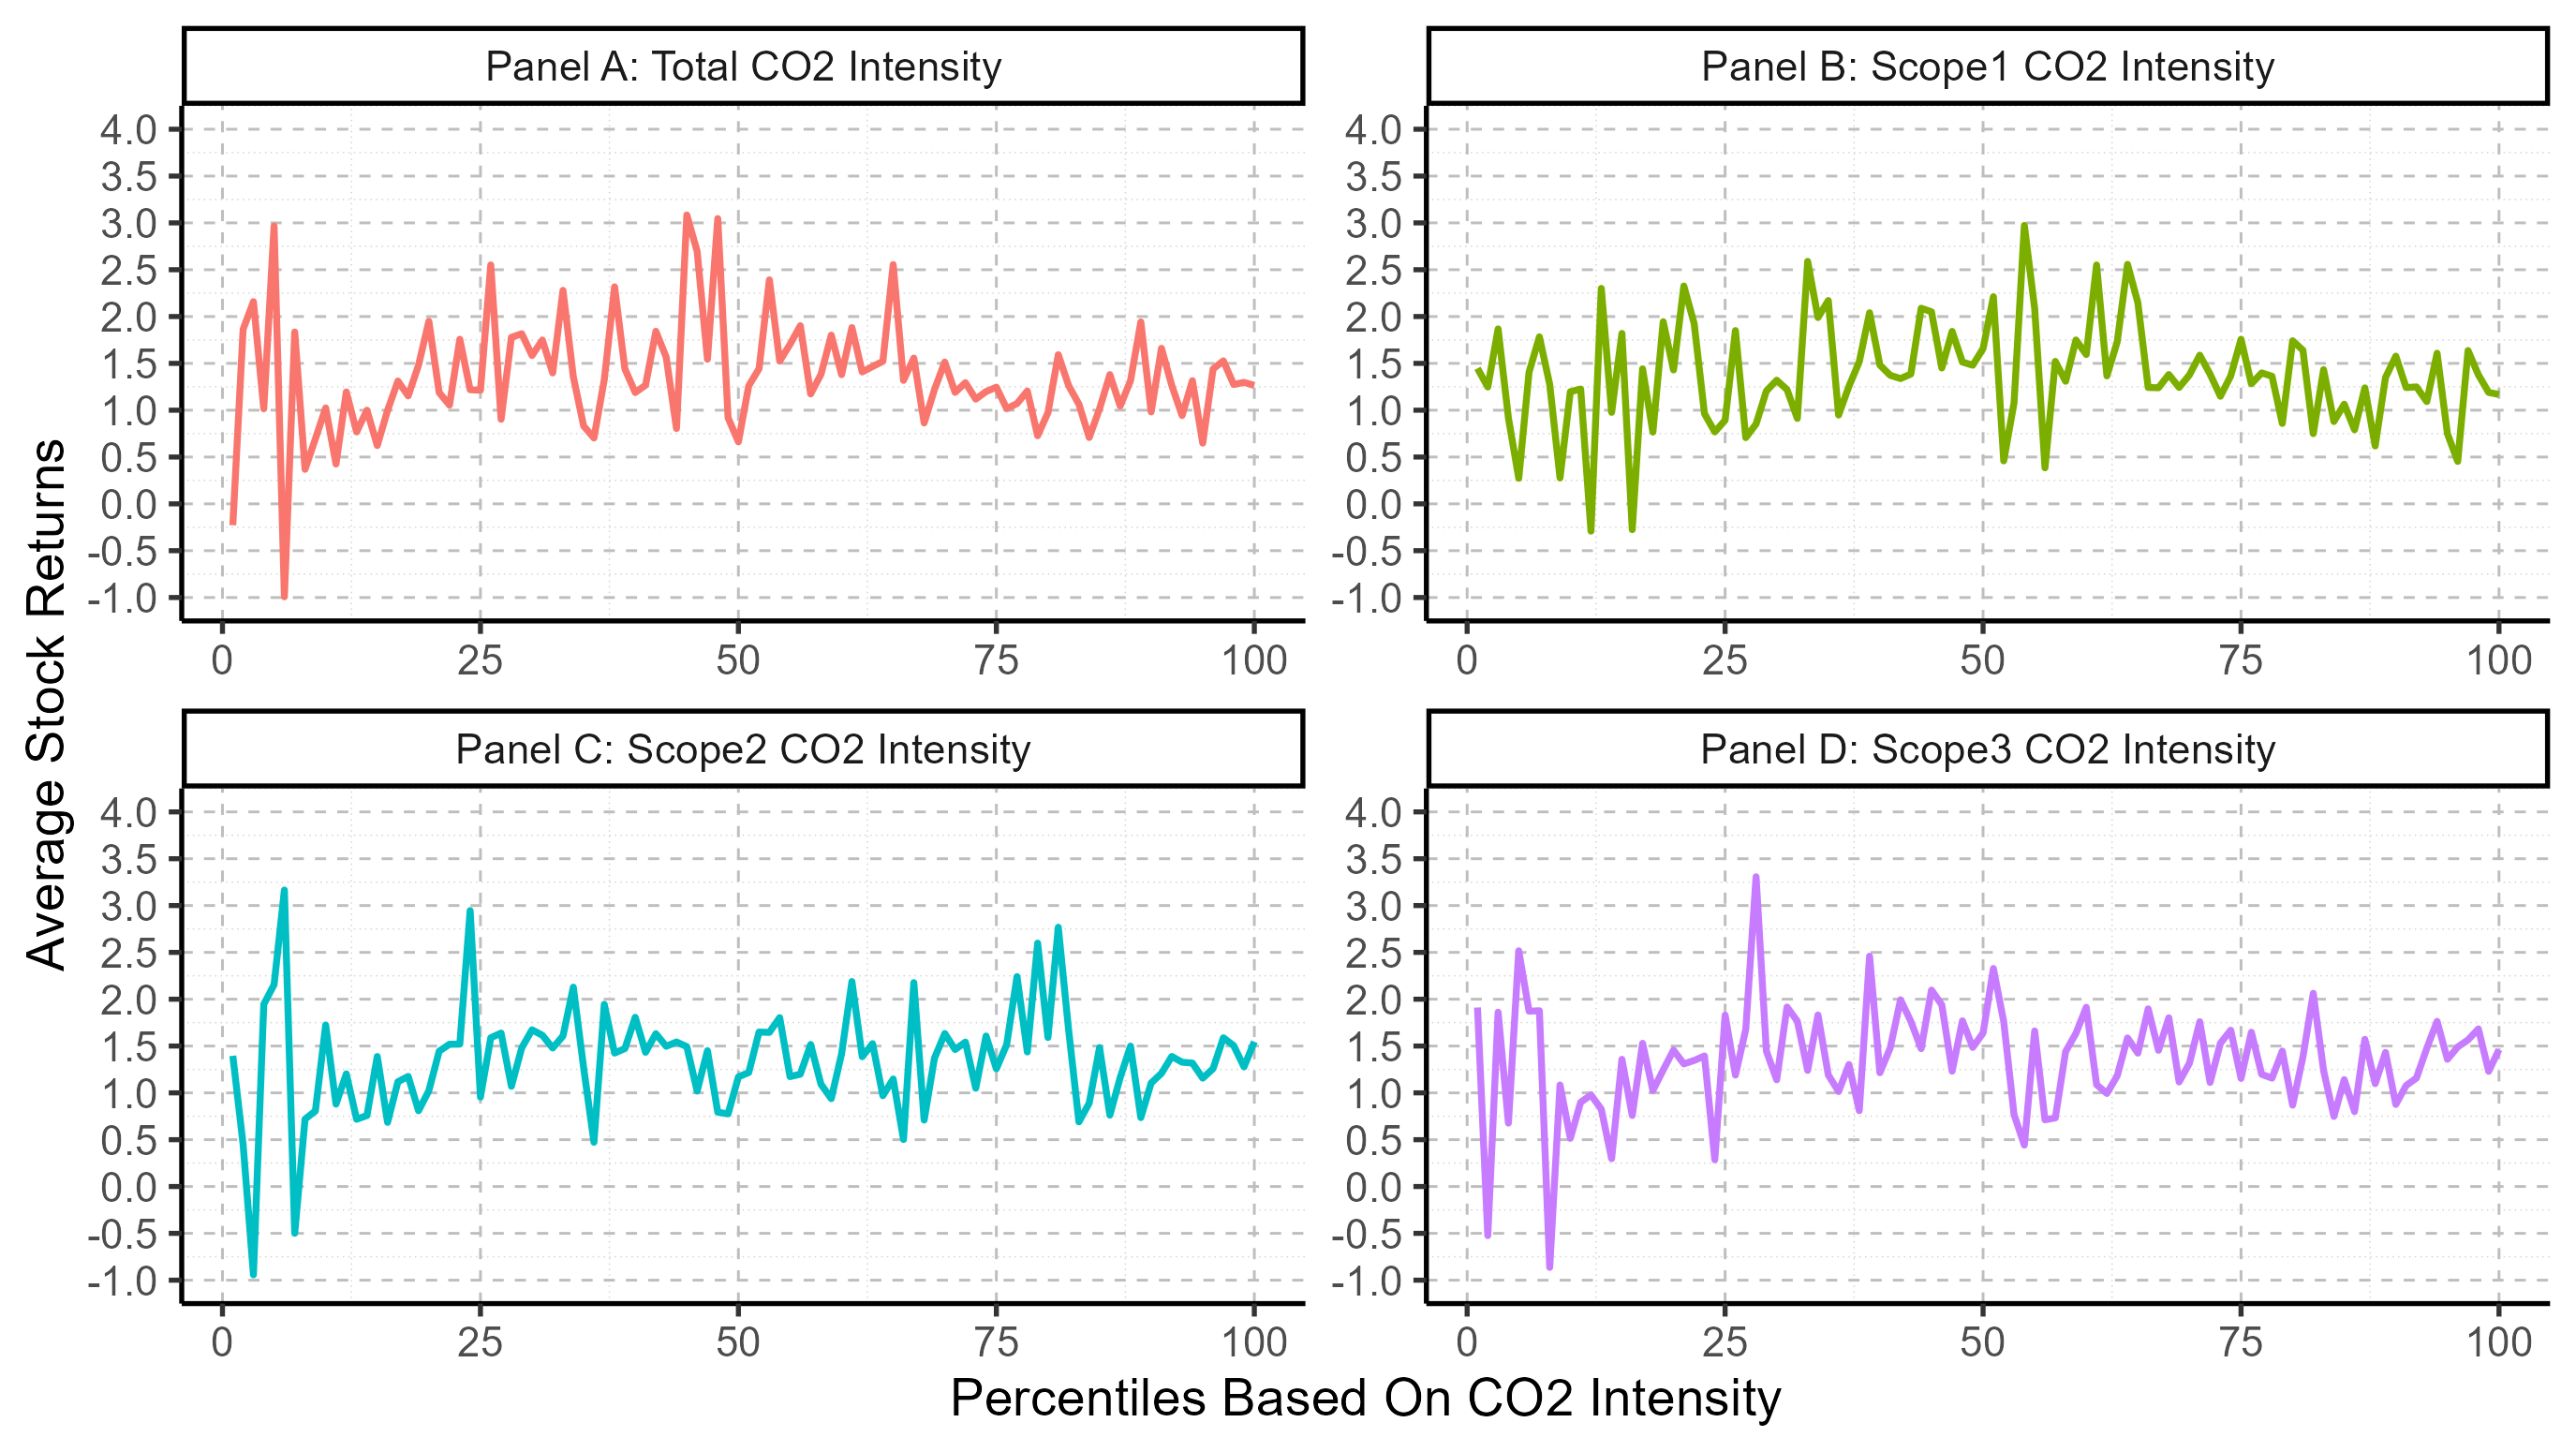
\includegraphics{image/intensity_percentile.png}
\label{fig: intensity_percentile}
\caption*{\footnotesize{This presents the average monthly stock returns in relation to different percentiles of CO2 intensity. Panel A depicts the average stock return in relation to firms' total CO2 intensity, while Panel B illustrates the average stock return concerning firms' scope 1 CO2 intensity. Panel C showcases the average stock return with respect to firms' scope 2 CO2 intensity, and Panel D presents the average stock return in connection with firms' scope 3 CO2 intensity.}}
\end{figure}

%%%%%%%%%%%%%%%%%%%%%%%%%%%%%%%%%%%%%%%%%%%%%%%%%%%
\subsection{Realized Cumulative Return for Green and Brown Portfolios}

Our following analysis involves constructing two distinct portfolios: a "Green" portfolio and a "Brown" portfolio, determined based on two carbon footprint indicators, namely total carbon emissions and carbon intensity. In general, firms with higher CO2 emissions and carbon intensity are often categorized as 'Brown' due to their significant environmental impact and contribution to carbon emissions. Hence, we categorize stocks into three percentiles based on firms' total carbon emissions, with firms exceeding the 66th percentile allocated to the Brown portfolio, and conversely, firms falling below the 33rd percentile assigned to the Green portfolio. Firms within the 33rd to 66th percentile range are placed in the Neutral portfolio. Furthermore, we repeat this procedure using carbon intensity as the criterion to classify stocks into Green, Neutral, and Brown portfolios. Subsequently, we comprehensively evaluate the performance of these portfolios, with cumulative portfolio returns graphically presented in Figures \ref{fig: cum_ret_1} and \ref{fig: cum_ret_2} over the period from 2002 to 2021. To ensure fairness and accuracy, each portfolio is weighted proportionally according to the size of the respective firms. It's important to note that portfolio reallocation occurs annually due to the annual update frequency of firms' carbon emission data, so the transaction fee can be ignored in this analysis.

\begin{figure}[!ht]
\centering
\caption{\textbf{Cumulative Green and Brown Portfolio Returns by CO2 Emissions}}
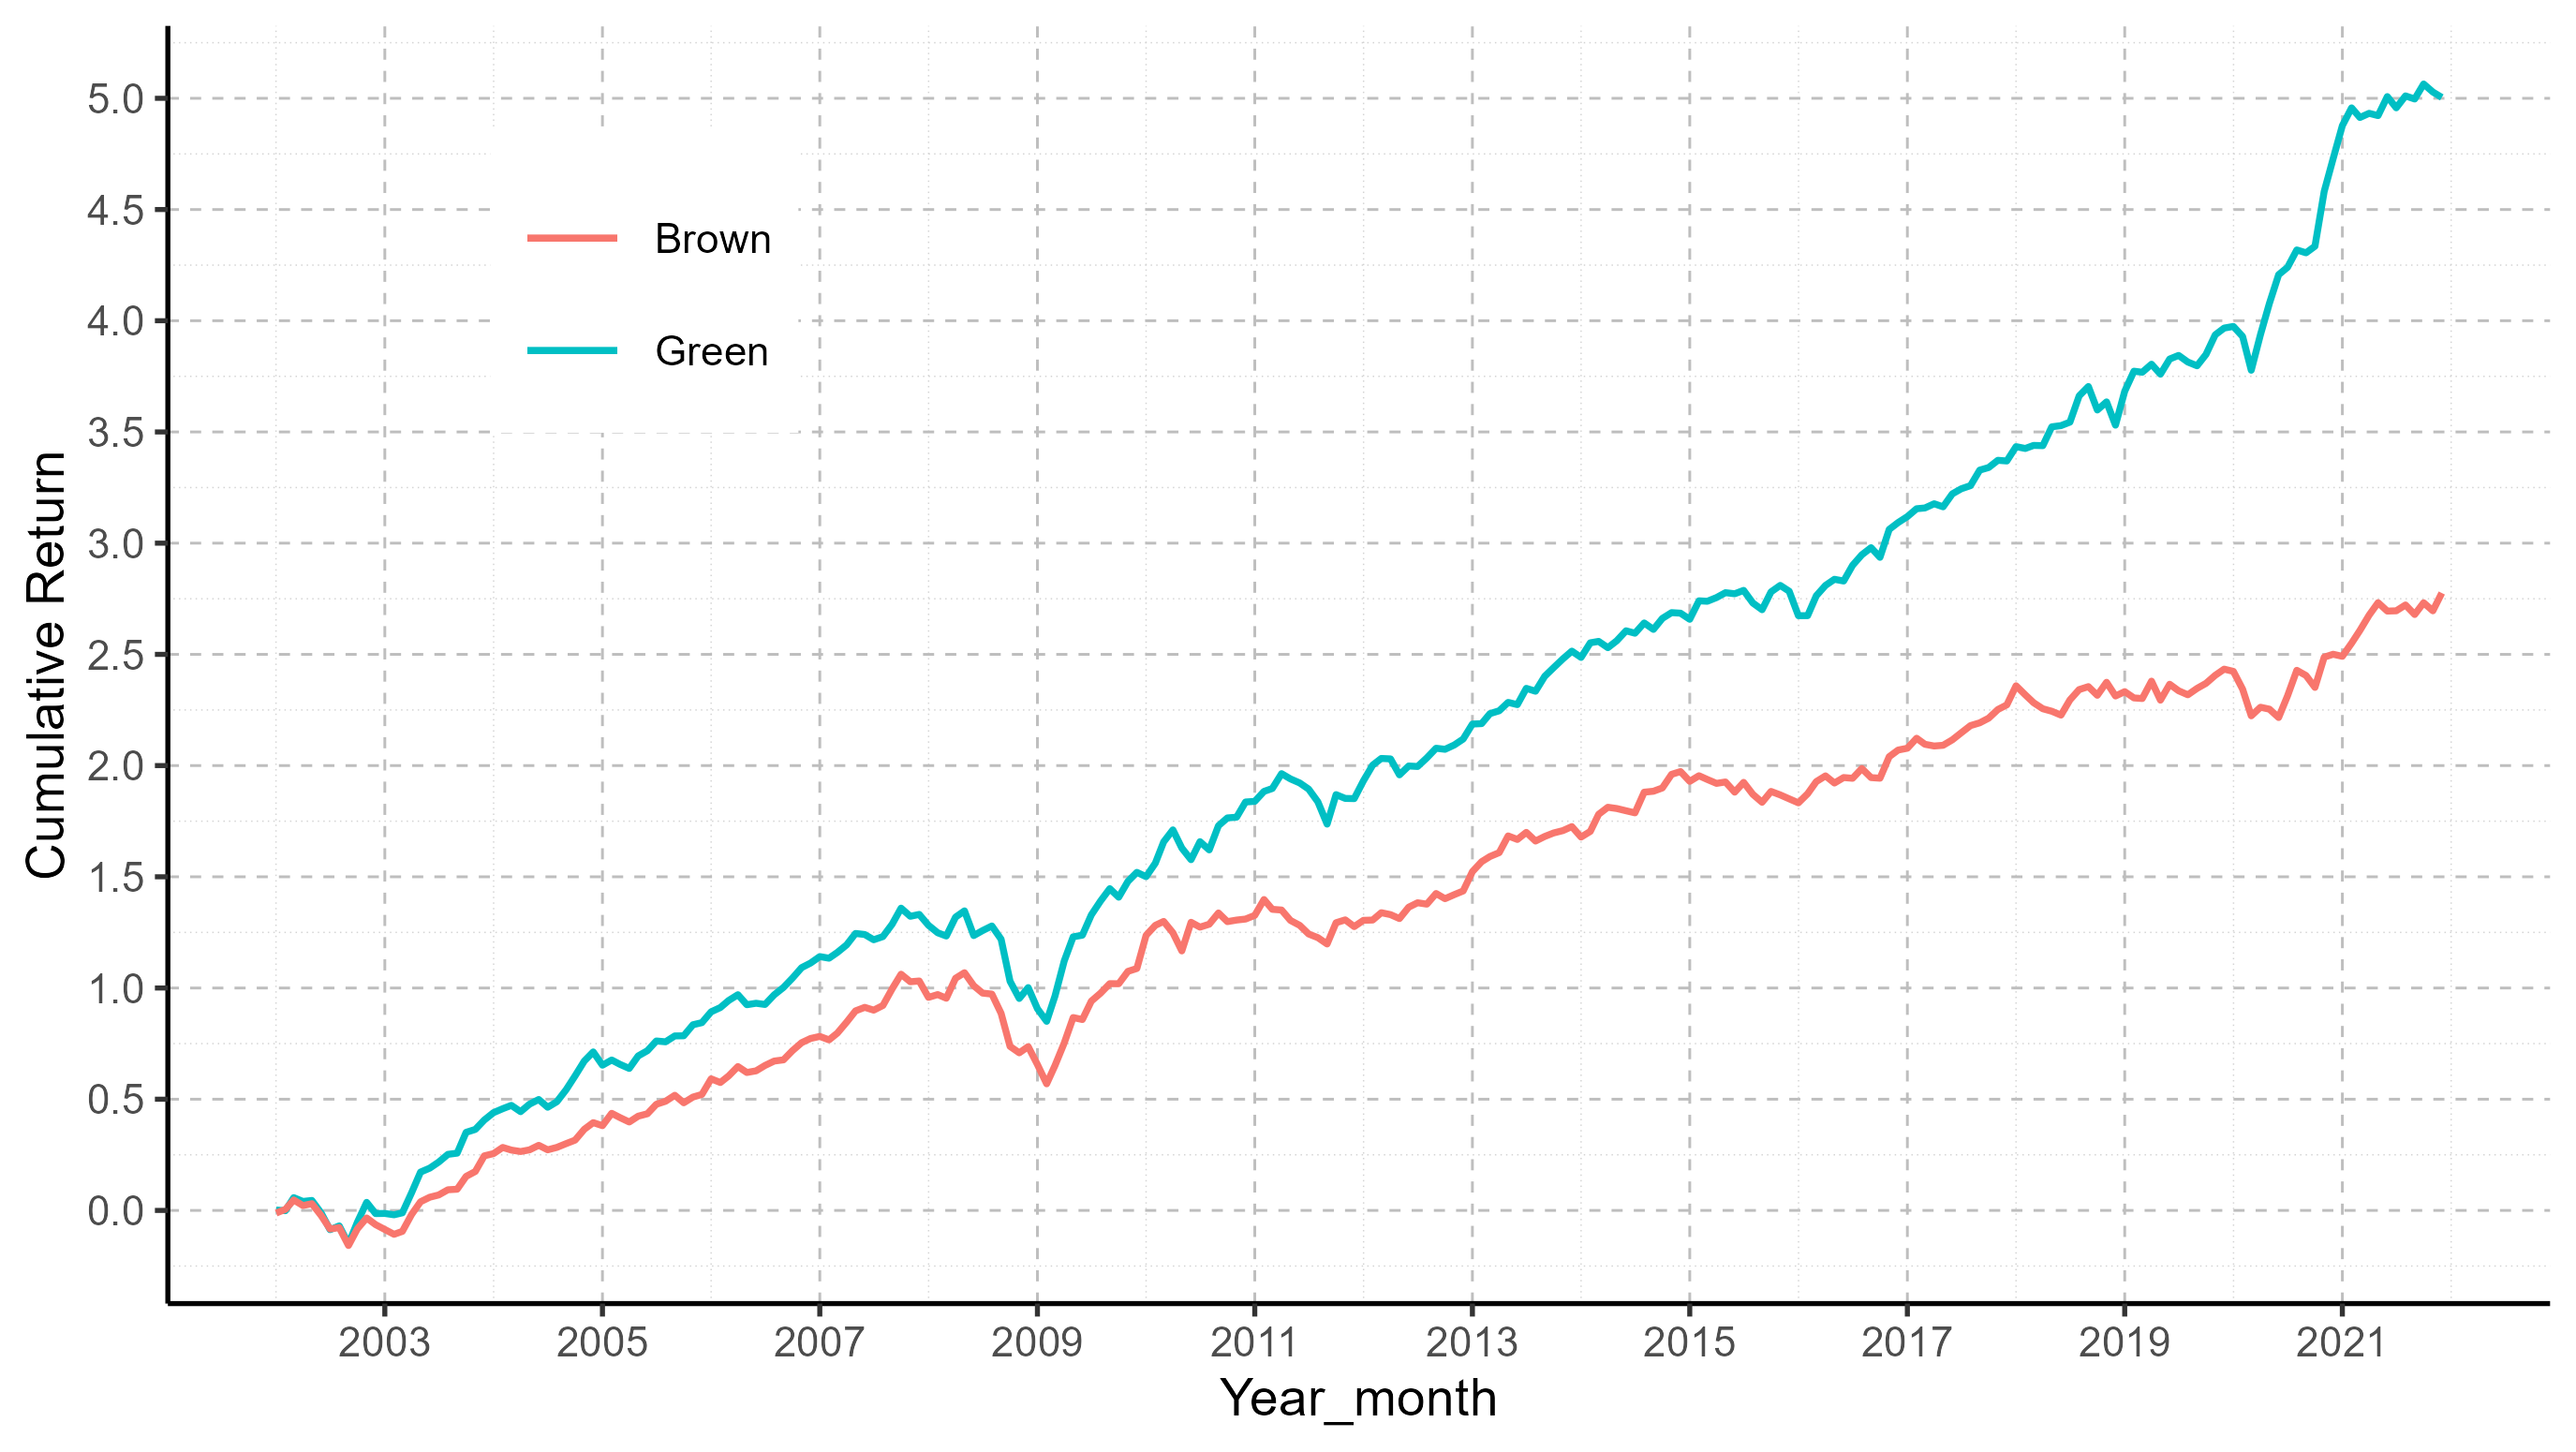
\includegraphics{image/green_brown_plot_1.png}
\label{fig: cum_ret_1}
\caption*{\footnotesize{This graphic illustrates the historical trajectory of firms' total CO2 emissions and intensity. Firms' total CO2 emissions are measured in thousand tons, while intensity is quantified by tons of CO2 emitted per million US dollars of revenue.}}
\end{figure}

When assessing companies based on their total CO2 emissions, the Green portfolio demonstrates superior performance over the Brown portfolio. This distinction is clearly evident in Figure \ref{fig: cum_ret_1}. The blue line in the graph represents the cumulative return of the green portfolio, which is based on firms' total CO2 emissions. Following this investment strategy until the end of our sample period results in an impressive cumulative return of over 500\% for the green portfolio. In contrast, employing the same investment strategy for the brown portfolio only leads to a cumulative return of less than 300\%. However, the scenario changes when we shift our focus to firms' CO2 intensity, as depicted in Figure \ref{fig: cum_ret_2}. In this case, the difference in performance between the Green and Brown portfolios is not as distinct. The Brown portfolio, represented by the orange line, consistently outperforms the green portfolio for a significant portion of the observed period. By the conclusion of our sample period, there is little disparity between the green and brown portfolios, as both have achieved approximately 300\% cumulative returns.

\begin{figure}[!ht]
\centering
\caption{\textbf{Cumulative Green and Brown Portfolio Returns by Intensity}}
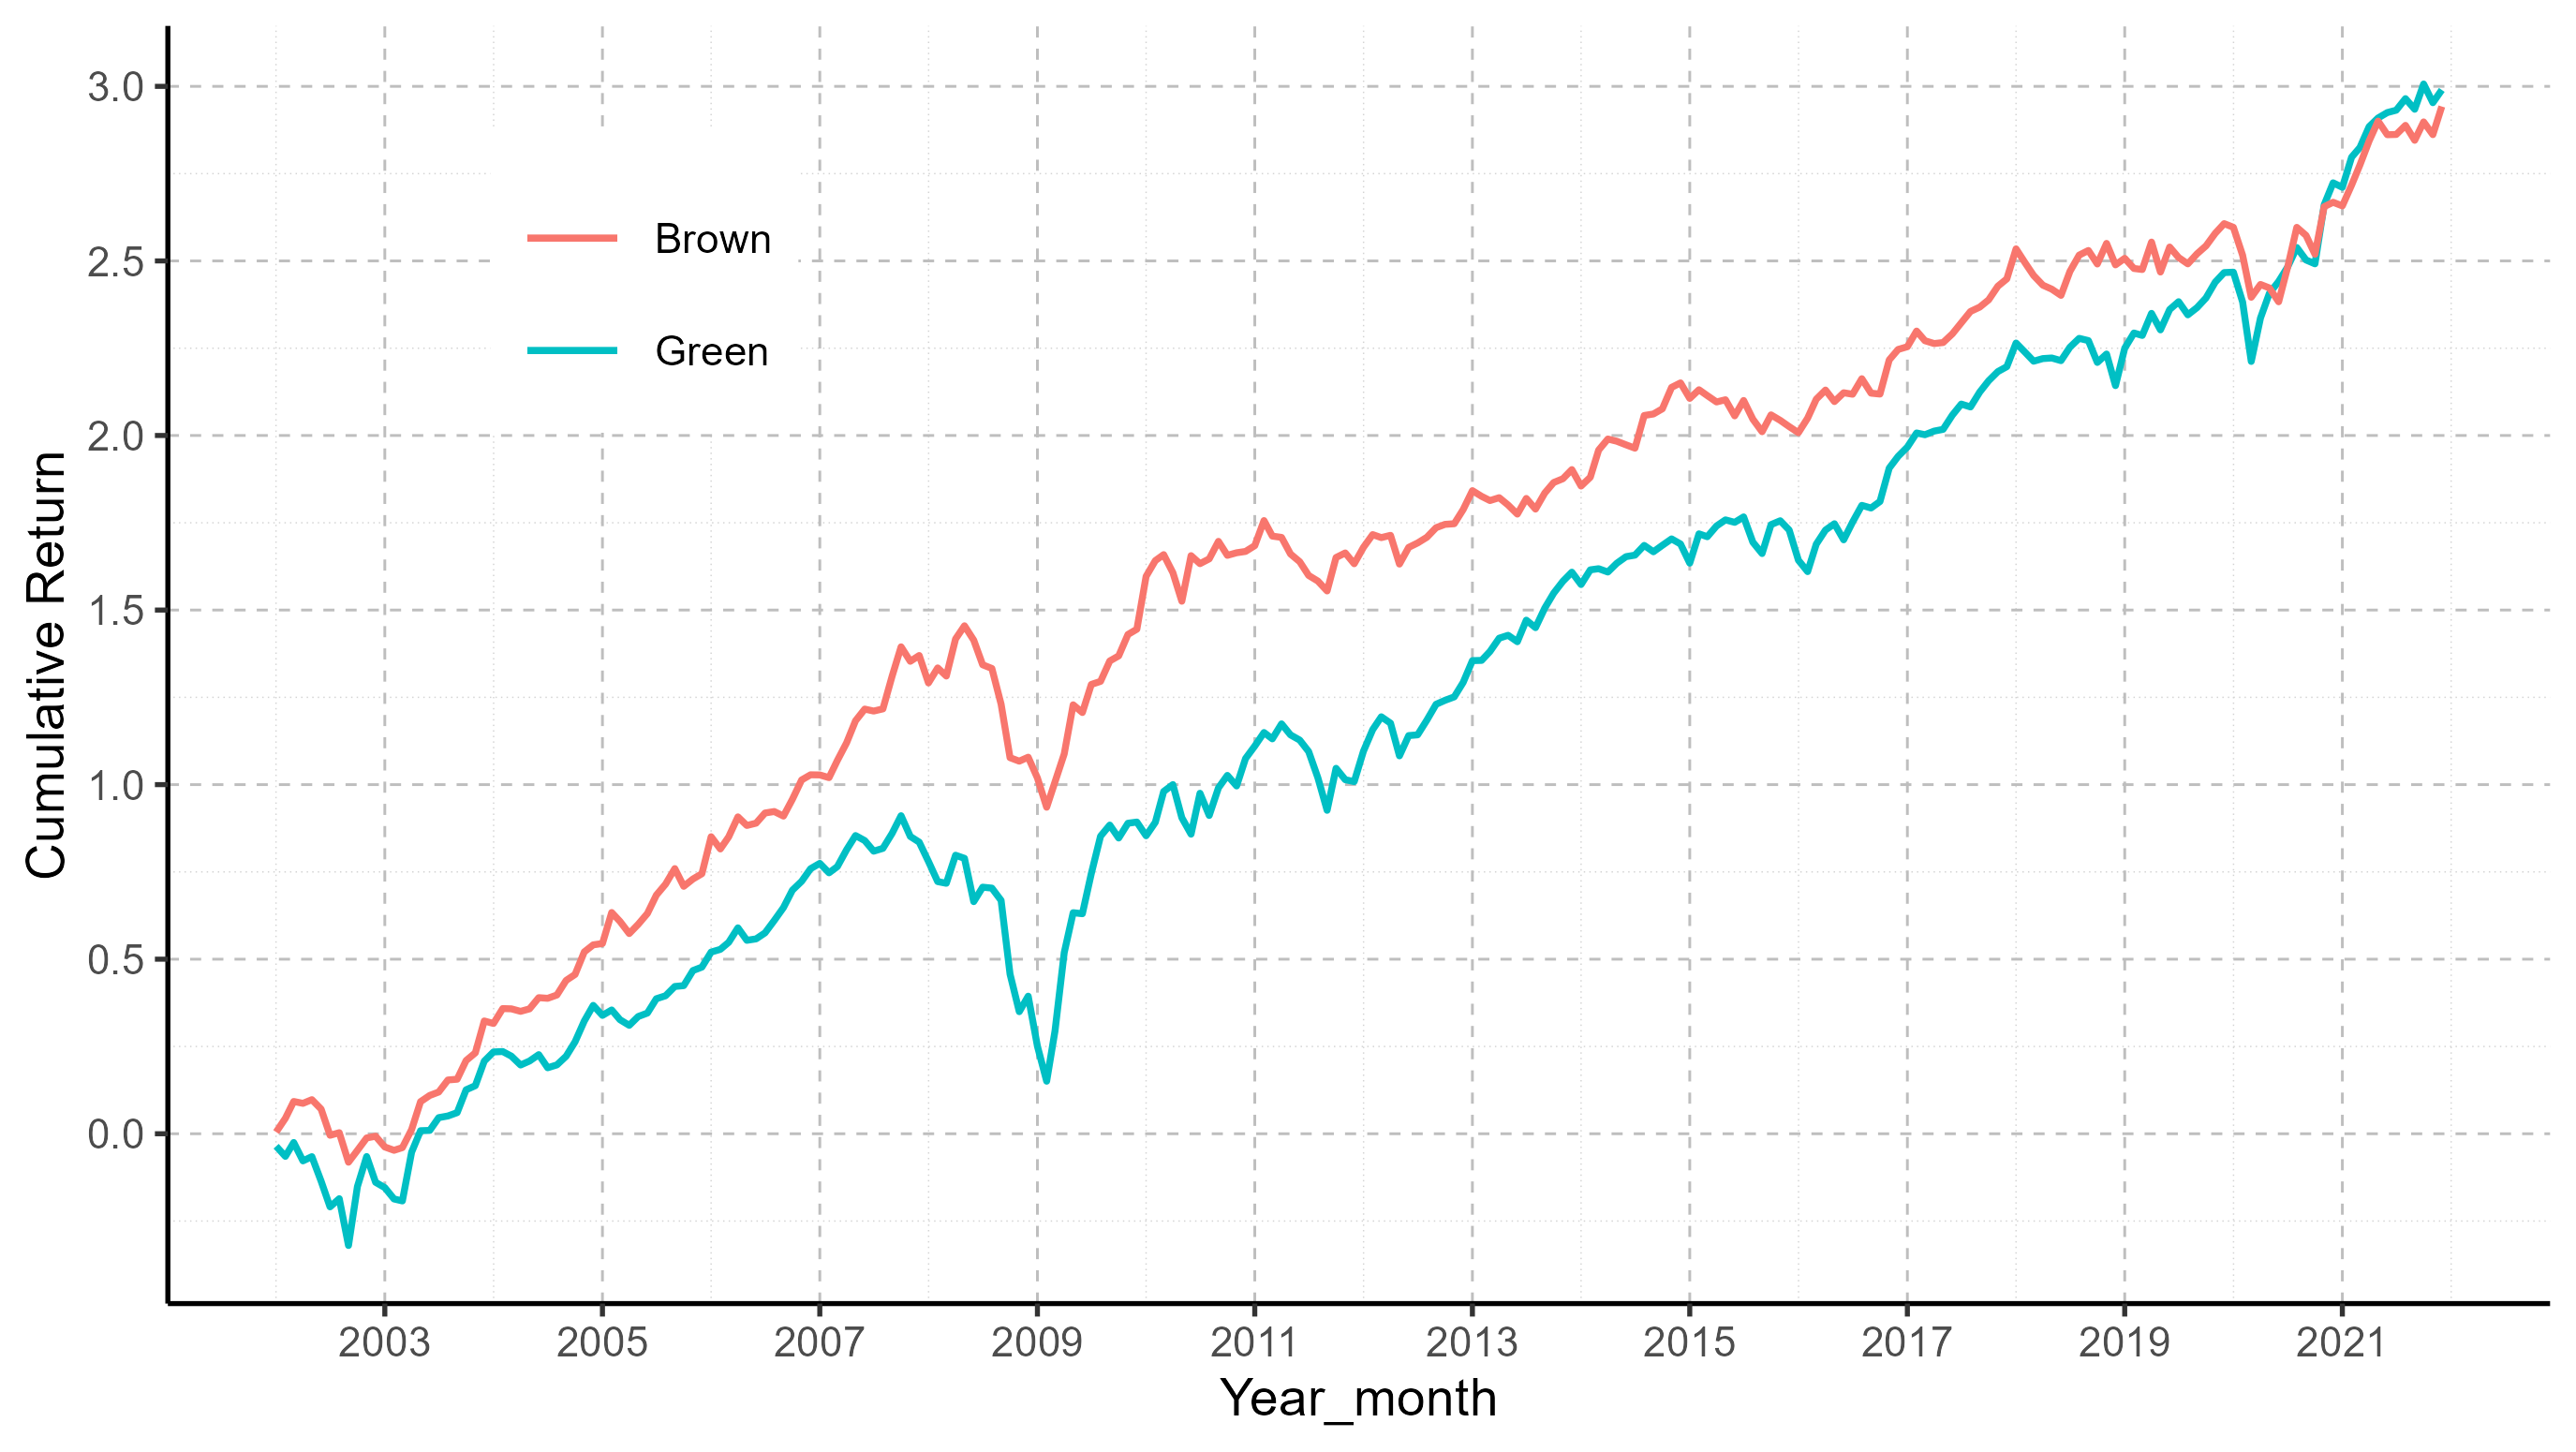
\includegraphics{image/green_brown_plot_2.png}
\label{fig: cum_ret_2}
\caption*{\footnotesize{This graphic illustrates the historical trajectory of firms' total CO2 emissions and intensity. Firms' total CO2 emissions are measured in thousand tons, while intensity is quantified by tons of CO2 emitted per million US dollars of revenue.}}
\end{figure}

%%%%%%%%%%%%%%%%%%%%%%%%%%%%%%%%%%%%%%%%%%%%%%%%%%%
\subsection{The Green-Brown Premium}

Taking inspiration from \cite{pastor2022dissecting}, we introduce the concept of the GMB (Green Minus Brown) premium, quantified as the monthly difference between the return of Green and Brown portfolios. This discrepancy is elaborated in Table \ref{tab: green-brown}, wherein the first column showcases the GMB premium originating from firms' overall CO2 emissions. Notably, the intercept is 44.3 basis points, accompanied by a corresponding standard error of 25.3 bp. This suggests that, on average, the Green portfolio outperforms the Brown counterpart by approximately 44.3 bp per month. Importantly, this difference exhibits statistical significance at the 10\% level. In contrast, the fourth column of Table \ref{tab: green-brown} elucidates the GMB premium derived from firms' CO2 intensity. Notably, in this case, the Green portfolio demonstrated no noteworthy outperformance against the Brown portfolio. The average stands at a mere 0.4 basis points per month, accompanied by a standard error of 26.3 bp, which is not significant either economically or statistically. 

In columns 2 and 3 of Table \ref{tab: green-brown}, we regress the GMB portfolio's return on the Fama-French 3 and 5 factors model, as discussed by \cite{fama2015five} and \cite{fama1993common}, the results show mixed evidence. With the Fama-French 5 factors model, we still get a significant positive intercept. This finding suggests that there is still an unexplained risk premium by the classical factor models. But with the Fama-French 3 factors model even if the intercept is still positive it becomes statistically insignificant.\footnote{In the paper by \cite{pastor2022dissecting}, they use E score from ESG rating to formulate GMB portfolio and find better empirical results, where all the intercepts are statistically and economically significant.} When we formulate the GMB portfolio by firms' CO2 intensity, all the intercepts from different regression models become both economically and statistically insignificant as shown in columns 4-6 in Table \ref{tab: green-brown}. The pivotal distinction between shaping the portfolio using total CO2 emissions versus intensity emerges as a noteworthy finding. Empirical evidence underscores the superiority of total CO2 emissions as a more robust indicator for quantifying firms' greenness. This empirical inclination emerges despite the seemingly logical construct of CO2 intensity. As it stands, the data does not substantiate CO2 intensity's position as a superior greenness indicator.
%%%%%%%%%%%%%%%%%%%%%%%%%%%%%%%%%%%%%%%%%%%%%%%%%%%

\begin{table}[!ht]
\centering
\footnotesize
\caption{Green - Brown Portfolios Regress on Factors}
\label{tab: green-brown}
{
\def\sym#1{\ifmmode^{#1}\else\(^{#1}\)\fi}
\begin{tabular}{@{\extracolsep{2pt}}l*{6}{c}@{}}
\toprule
& \multicolumn{3}{c}{CO2 Emission} & \multicolumn{3}{c}{Intensity} \\
\cline{2-4}
\cline{5-7}
 & (1) & (2) & (3) & (4) & (5) & (6) \\
\hline
Intercept & 0.443\sym{*} & 0.193 & 0.405\sym{*} & 0.004 & -0.280 & -0.004 \\
 & (0.253) & (0.224) & (0.229) & (0.263) & (0.248) & (0.250) \\
Mkt-RF &  & 0.128\sym{**} & 0.069 &  & 0.323\sym{***} & 0.248\sym{***} \\
 &  & (0.054) & (0.056) &  & (0.060) & (0.062) \\
SMB &  & 0.705\sym{***} & 0.625\sym{***} &  & 0.149 & 0.021 \\
 &  & (0.095) & (0.097) &  & (0.105) & (0.106) \\
HML &  & -0.351\sym{***} & -0.249\sym{***} &  & -0.037 & 0.053 \\
 &  & (0.084) & (0.093) &  & (0.093) & (0.102) \\
RMW &  &  & -0.359\sym{***} &  &  & -0.536\sym{***} \\
 &  &  & (0.113) &  &  & (0.123) \\
CMA &  &  & -0.192 &  &  & -0.054 \\
 &  &  & (0.149) &  &  & (0.163) \\

\hline
Obs & 240 & 240 & 240 & 240 & 240 & 240 \\
Adj. R\sym{2} & 0.000 & 0.245 & 0.273 & -0.000 & 0.137 & 0.194 \\
\bottomrule
\multicolumn{7}{l}{\footnotesize * p\sym{<}.1, ** p\sym{<}.05, *** p\sym{<}.01}
\end{tabular}
}
\begin{tablenotes}
    \item This table presents the regression results of the Green minus Brown portfolio on different factor models. In the left panel, the portfolio is formulated based on firms' total CO2 emissions, and in the right panel, the portfolio is based on firms' CO2 intensity. Columns 1 and 4 only show regression results with intercept, columns 2 and 5 show regression results with Fama-French 3 factors model, and columns 3 and 6 show regression results with Fama-French 5 factors model.
\end{tablenotes}
\end{table}

%%%%%%%%%%%%%%%%%%%%%%%%%%%%%%%%%%%%%%%%%%%%%%%%%%%
\subsection{The Influence of Climate Concerns}

As outlined in the equilibrium model developed by \cite{pastor2021sustainable} and \cite{pedersen2021responsible}, an intriguing dynamic unfolds. In times of heightened climate concern, green stocks emerge as beneficiaries, securing elevated anticipated returns. This positive trajectory reflects the growing investor preference for environmentally conscientious options. Conversely, the brown stocks face a contrasting fate, experiencing a dip in their projected returns. This downturn aligns with investors' inclination to retreat from these stocks amid escalated climate concerns. 

Next, We are going to test this result empirically by using regression analysis, wherein we regress GMB, Green, Brown, and Neutral portfolios on UMC (unexpected media climate change concerns) constructed by \cite{ardia2022climate}\footnote{It's important to note a slight difference in the construction of UMC in this paper compared to \cite{ardia2022climate}. While they employ a different set of control variables, including the Fama-French 5 factors, momentum factor, WTI return, gas return, propane return, U.S. economic policy uncertainty index, VIX, TED spread, term factor, default factor, etc.}. Our UMC index construction follows the same approach as \cite{ardia2022climate}, utilizing an ARX model. However, we incorporate different control variables in our model, including the Fama-French 5 factors, CFNAI index, investor sentiment, WTI index, VIX index, and a lagged one-period MCCC index to compute UMC. Specifically, our model for MCCC is specified as $MCCC_t = \alpha + \beta MCCC_{t-1} + \gamma Controls_{t-1} + \epsilon$, with $UMC_t = MCCC_t - \widehat{MCCC_t}$. For a more detailed description of the MCCC (Media Climate Change Concern) index, please refer to Appendix \ref{sec: mcc}. The regression incorporating the UMC index for the Green and Brown portfolios is outlined as follows:

\begin{equation}
    RET_t = \alpha_t + \beta_1 UMC_t + \beta_2 Controls_t + \epsilon_t
\label{eqn: test_pastor_model}
\end{equation}
where $RET_t$ represents portfolio's return, $UMC_t$ is unexpected media climate change concerns, and $Contorls_t$ is a list of control variables including Fama-French 5 factors, CFNAI index (Chicago Fed National Activity Index constructed), investor sentiment (constructed by \cite{baker2007investor}, WTI index (Crude Oil WTI price), and VIX index (Chicago Board Options Exchange's CBOE Volatility Index). And we expect that $\beta^{GMB}_1$ and $\beta^{Green}_1$ are both positive, $\beta^{Brown}_1$ is negative, and $\beta^{Neutral}_1$ is insignificant.

%%%%%%%%%%%%%%%%%%%%%%%%%%%%%%%%%%%%%%%%%%%%%%%%%%%
\begin{table}[H]
\centering
\footnotesize
\caption{Green - Brown on UMC}
\label{tab: on_umc}
{
\def\sym#1{\ifmmode^{#1}\else\(^{#1}\)\fi}
\begin{tabular}{@{\extracolsep{2pt}}l*{4}{c}@{}}
\toprule
& \multicolumn{4}{c}{Dependent Variable}\\
\cline{2-5}
 & Green-Brown & Green & Brown & Neutral \\
\hline
Intercept & 0.014 & 0.473 & 0.459 & 0.623\sym{*} \\
 & (0.979) & (0.408) & (0.870) & (0.372) \\
UMC & 1.493\sym{*} & 0.226 & -1.266\sym{*} & 0.187 \\
 & (0.855) & (0.356) & (0.759) & (0.324) \\

\hline
Controls & Yes & Yes & Yes & Yes \\
Obs & 227 & 227 & 227 & 227 \\
Adj. R\sym{2} & 0.282 & 0.901 & 0.522 & 0.919 \\
\bottomrule
\multicolumn{5}{l}{\footnotesize * p\sym{<}.1, ** p\sym{<}.05, *** p\sym{<}.01}
\end{tabular}
}
\begin{tablenotes}
    \item This table represents the regression results of Green-Brown, Green, Brown, and Neutral portfolios on the UMC index and a group of control variables. \citet{ardia2022climate} constructed the MCCC index since January 2003, hence the number of observations is less than 240. The Green Portfolio contains firms with total CO2 emissions up to the 33rd percentile, Neutral Portfolio contains firms with total CO2 emissions ranging from the 34th to 66th percentile, and firms with CO2 emissions higher than the 66th percentile are included in the Brown Portfolio. Green-Brown Portfolio is the monthly difference between Green and Brown portfolios.
\end{tablenotes}
\end{table}

Presented in Table \ref{tab: on_umc}, the regression findings illuminate the outcomes of diverse portfolios structured based on firms' CO2 emissions in relation to the UMC index, accompanied by a set of control variables as specified by Equation \ref{eqn: test_pastor_model}. Upon examination, our initial observation surfaces: all portfolios, except for the Neutral portfolio\footnote{It's important to clarify that the neutral portfolio does not signify null CO2 emissions. Instead, firms within this portfolio exhibit total carbon emissions ranging between the 34th and 66th percentiles across the entire sample.}, showcase statistically insignificant intercepts. This suggests that the incorporation of the UMC index adeptly explains the returns across all portfolios. In the first column, notable trends emerge. The Green-Brown portfolio reveals its potential to accrue an average increase of 1.39\% in returns with each unit augmentation in the UMC index. This effect holds significant at the 1\% level. Contrarily, the third column captures the Brown portfolio's response, indicating an average decrease of -1.27\% in returns per unit uptick in the UMC index. Intriguingly, the UMC coefficient for the Neutral portfolio fails to achieve significance, indicating that the UMC index does not have a marginal influence on its returns. Lastly, in the second column, while a positive correlation between the Green portfolio and the UMC index aligns with our expectations, unfortunately, we do not observe significant statistical evidence to support our hypothesis.

%%%%%%%%%%%%%%%%%%%%%%%%%%%%%%%%%%%%%%%%%%%%%%%%%%%

%%%%%%%%%%%%%%%%%%%%%%%%%%%%%%%%%%%%%%%%%%%%%%%%%%%
\subsection{Firm Level Evidence}

In the previous section, we constructed Green and Brown portfolios based on firms' total CO2 emissions. Interestingly, our findings showcased the Green portfolio's consistent outperformance over the Brown portfolio, particularly in the presence of high unexpected climate concerns (UMC). This trend appears to diverge from the conclusions drawn by \cite{bolton2021investors}, who, employing firm-level data, reveal a contrasting pattern. Their study highlights that firms characterized by higher carbon emissions (referred to as Brown firms in our context) tend to yield greater realized stock returns. Their interpretation centers around the integration of the climate risk premium within these returns. This notion indicates that investors factor in the associated climate risk, and require compensation from firms with higher climate risk exposure (firms with higher CO2 emissions). As per their reasoning, elevated CO2 emissions are linked with heightened climate risk, thus justifying the anticipation of a commensurately higher risk premium. In this section, we aim to critically revisit the empirical evidence from firm-level analysis.

To decipher the intricate relationship between companies' total CO2 emissions and their stock returns, we utilize a robust approach. We undertake the estimation of a time series regression model using Panel OLS:

\begin{equation}
    \label{eqn: firm_level}
    RET_{i,t} = \alpha + \beta_1 CO2\_tot_{i,t} + \beta_2 Contorls_{i,t} + \epsilon_{i,t}
\end{equation}

Here, $RET_{i,t}$ represents the stock return of firm $i$ during month $t$, and $CO2_{tot}$ corresponds to firms' total CO2 emissions, scaled logarithmically. The vector $Controls_{i,t}$ encompasses a range of control variables, encompassing firm-specific factors known for their predictive influence on returns. These variables include firm size (logged), leverage (total liability divided by total assets), B/M (book-to-market ratios), RoE (return on equity), Inves/AT (investment scaled by total assets), PPE (Property, plant, and equipment, logged), SaleGR (sales growth), EPS (earnings per share), Staff\_num (number of staff, logged), and Firm\_age (years since foundation). Our primary focus lies in interpreting the coefficient $\beta_1$, which plays a pivotal role in our investigation.

%%%%%%%%%%%%%%%%%%%%%%%%%%%%%%%%%%%%%%%%%%%%%%%%%%%
\subsubsection{Benchmark Result}

Based on Equation \ref{eqn: firm_level}, the findings are presented in Table \ref{tab: firm_level}, showcasing the results of firm-level analysis across two different fixed effects specifications for both the restricted and unrestricted models. In our approach, we use time-fixed effects at the month level. This choice serves to mitigate the impact of temporal variations across time, including broader economic conditions, shifts in investors' sentiments towards the stock market, the evolving concern for climate change, and other time-dependent factors. Columns 1 and 2 elucidate the outcomes of the regression analysis for the unrestricted and restricted models, respectively, incorporating Time + Industry two-way fixed effects. Notably, these techniques align with the methodologies employed by \cite{bolton2021investors}. By integrating industry-fixed effect, we effectively control for variations across distinct industries. This approach permits us to find the average correlation between firms' total CO2 emissions and stock return cross-sectionally without the influence to which industry a firm belongs. 

For the unrestricted model presented in column 1, we find a positive correlation between firms' total CO2 emissions and stock return, However, the near-zero R-squared value indicates limited explanatory power, potentially attributed to omitted variables. Moving to column 2, the restricted model's outcomes are showcased. The consistent positive relationship between firms' total CO2 emissions and stock returns persists but loses statistical significance. Different from \cite{bolton2021investors} paper, where they get significant results between stock return and various scopes of CO2 emissions by excluding firms from salient industries (GIC 19, 20, 23), here we analyze all the firms regardless of which industry they belong to. Furthermore, an additional consideration raised by \cite{aswani2023carbon} involves the potential for collinearity between firm size and CO2 emissions. They argue that the apparent positive link between CO2 emissions and stock returns might be influenced by this collinearity. There is no doubt that larger firms tend to have more CO2 emissions, and industry-level fixed effects can not identify this collinearity issue.

Columns 3 and 4 in Table \ref{tab: firm_level} showcase the un/-restricted model with Time + Entity (firm) two-way fixed effects. Different from Time + Industry two-way fixed effects, with Time + Entity fixed effects the analysis considers both time-specific variations and variations unique to individual entities (firms). By including Entity fixed effects, we are accounting for firm-specific factors that may be constant over time but vary across different firms. This is a more stringent restriction by the assumption that investors not only distinguish industry-specific characteristics but also place a heightened emphasis on each firm's specific inherent attributes. 

First, it is important to note that the results remain consistent between the un-/restricted models presented in columns 3 and 4. Then, the most intriguing revelation arises from the incorporation of Time + Entity two-way fixed effects, leading to an observed sign reversal of the coefficient on CO2 emissions. This shift takes place under the assumption that investors place greater emphasis on each firm's intrinsic attributes rather than industry-specific characteristics. Specifically, firms with higher CO2 emissions, implying increased exposure to climate risks, tend to exhibit lower stock returns on average. Importantly, this observation maintains both economic and statistical significance. And it's important to underscore that this finding aligns with the persistent outperformance of the Green portfolio over the Brown portfolio. Finally, given that the positive relationship between firm size and stock returns persists, concerns of collinearity between CO2 emissions and firm size in predicting stock returns, as brought up by \cite{aswani2023carbon} are no longer applicable.\footnote{Table \ref{tab: corr} shows there is a positive correlation between firms' CO2 emissions and their size, but the relationship between return and CO2 emissions has an opposite sign to the relationship between return and size.}


\begin{table}[H]
\centering
\footnotesize
\caption{Firm Level Analysis}
\label{tab: firm_level}
{
\def\sym#1{\ifmmode^{#1}\else\(^{#1}\)\fi}
\begin{tabular}{@{\extracolsep{2pt}}l*{4}{c}@{}}
\toprule
& \multicolumn{4}{c}{Returns} \\
\cline{2-5}
 & (1) & (2) & (3) & (4) \\
\hline
CO2\_tot & 0.075\sym{*} & 0.034 & -0.176\sym{**} & -0.659\sym{***} \\
 & (0.040) & (0.053) & (0.090) & (0.127) \\
Size &  & 0.250\sym{**} &  & 1.535\sym{***} \\
 &  & (0.101) &  & (0.197) \\
Levarage &  & -0.226 &  & 0.173 \\
 &  & (0.203) &  & (0.422) \\
B/M &  & -1.879\sym{***} &  & -2.729\sym{***} \\
 &  & (0.181) &  & (0.276) \\
RoE &  & 0.526\sym{***} &  & 0.292\sym{***} \\
 &  & (0.086) &  & (0.101) \\
Inves/AT &  & -4.447\sym{***} &  & -12.650\sym{***} \\
 &  & (1.132) &  & (1.874) \\
PPE &  & -0.008 &  & -0.426\sym{***} \\
 &  & (0.048) &  & (0.162) \\
SaleGR &  & 0.916\sym{***} &  & 0.799\sym{***} \\
 &  & (0.224) &  & (0.237) \\
EPS &  & 0.057\sym{***} &  & 0.018 \\
 &  & (0.022) &  & (0.027) \\
Staff\_num &  & -0.278\sym{***} &  & -0.835\sym{***} \\
 &  & (0.066) &  & (0.213) \\
Firm\_age &  & -0.047 &  & 1.789\sym{***} \\
 &  & (0.065) &  & (0.517) \\
Constant & 0.162 & 0.526 & 3.353\sym{***} & -3.421 \\
 & (0.505) & (0.643) & (1.137) & (2.940) \\

\hline
Firm F.E. & No & No & Yes & Yes \\
Industry F.E. & Yes & Yes & No & No \\
Year-Month F.E. & Yes & Yes & Yes & Yes \\
\hline
Obs & 466999 & 295704 & 466999 & 295704 \\
R-squared & 0.000 & 0.013 & 0.000 & 0.019 \\
\bottomrule
\multicolumn{5}{l}{\footnotesize * p\sym{<}.1, ** p\sym{<}.05, *** p\sym{<}.01}
\end{tabular}
}
\begin{tablenotes}
    \item This table presents the regression results depicting the influence of firms' CO2 emissions on stock returns. To account for potential dependencies within the data, the standard errors are clustered at the specified level along with the fixed effects integrated into the model.
\end{tablenotes}
\end{table}

%%%%%%%%%%%%%%%%%%%%%%%%%%%%%%%%%%%%%%%%%%%%%%%%%%%
\subsubsection{Robustness Check}

In the context of the regression model \ref{eqn: firm_level}, the choice of fixed effects can vary depending on the underlying assumptions. In conventional cross-sectional stock return analyses, it is a common practice to assume significant heterogeneity between industries, with the belief that firms within a particular industry exhibit similar characteristics in terms of their stock returns. This assumption has garnered substantial empirical support in the existing literature. However, it's crucial to recognize that investors base their investment allocation decisions on more than just industry categorizations. While they may initially screen industries, their ultimate investment choices often depend on the specific attributes of individual companies. In such scenarios, even firms within the same industry can exhibit significant variations in their stock performance. Therefore, considering heterogeneity at the firm level may be a more suitable approach than relying solely on industry-level assumptions. In the following analysis, we perform a robustness check with various fixed effects and cluster standard errors at different levels.

The first six models depicted in Figure \ref{fig: forestplot} include the benchmark model along with variations involving different fixed effects. In the case of considering only the Entity fixed effect, we observe a coefficient of -0.74 for total CO2 emissions, which is statistically significant at the 1\% level. Similarly, when we incorporate both Entity and Year two-way fixed effects, the CO2 emissions coefficient remains statistically significant at the 1\% level, with a slightly reduced value of -0.72. These specifications maintain consistency with the benchmark model, showing only minor coefficient adjustments. Moving on to models 4, 5, and 6, where we introduce industry fixed effects, industry + year-month, and industry + year two-way fixed effects, we observe a different pattern. In these models, the coefficients on CO2 emissions all become statistically insignificant and approach zero.

\cite{white1980heteroskedasticity} in his seminar paper first introduced Robust standard errors in econometrics to account for heteroscedasticity. In Model \ref{eqn: firm_level}, which retains the same fixed effects as the benchmark model, the application of robust standard errors significantly increases statistical significance and narrows down the confidence intervals as depicted by the 7th model in Figure \ref{fig: forestplot}. Furthermore, as highlighted by \cite{petersen2008estimating}, in corporate and empirical and asset pricing research, when dealing with panel data the residuals may be correlated across firms or across time. In such cases, standard errors can be biased. To mitigate this, Petersen recommends clustering standard errors at the same level, as is done in our benchmark model. Additionally, \cite{angrist2009mostly} advocates for clustering standard errors at a level one step above the sample data. In line with this recommendation, we cluster the standard errors at the industry and year level for the benchmark model to test its robustness. After applying clustering to standard errors at the Industry + Year level, we observe a slight increase in standard errors compared to the benchmark model. Nonetheless, the results remain statistically significant at the 1\% level, as shown by the last model in Figure \ref{fig: forestplot}.

%%%%%%%%%%%%%%%%%%%%%%%%%%%%%%%%%%%%%%%%%%%%%%%%%%%
\begin{figure}[H]
\centering
\caption{\textbf{Change of Fixed Effects and Cluster Levels}}
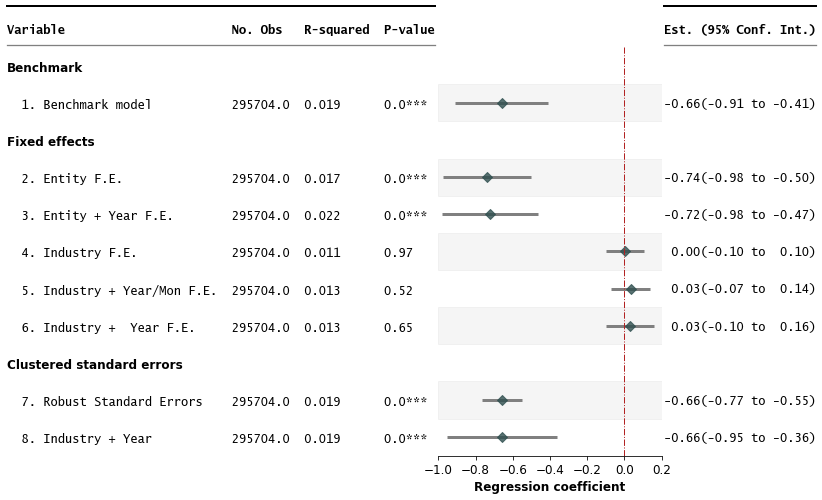
\includegraphics[width=.8\textwidth]{image/forestplot.png}
\label{fig: forestplot}
\caption*{\footnotesize{This graphic presents coefficients and associated confidence intervals for various fixed effects and clustered standard error configurations. The benchmark model includes Entity + Year/Month fixed effects, with standard errors clustered at the same level. In the 'Fixed Effects' group, we explore different fixed effects for each model, while maintaining standard errors clustered at the same level. In the 'Clustered Standard Errors' group, we examine how standard errors are clustered at various levels while keeping the fixed effects consistent with the benchmark model.}}
\end{figure}

%%%%%%%%%%%%%%%%%%%%%%%%%%%%%%%%%%%%%%%%%%%%%%%%%%%
\subsubsection{Interplay with climate concerns}
In the previous section, we find a negative relationship between firms' CO2 emissions and their stock returns when using Time + Entity two-way fixed effects. This finding holds true under the assumption that investors not only differentiate between industry-specific characteristics but also place significant emphasis on the unique characteristics of each firm. The reason behind this relationship may be linked to investors' growing commitment to green investing mandates and their increasing concerns about the potential risks posed by climate change. Consequently, it becomes intriguing to delve into the dynamic between a firm's CO2 emissions and public climate concerns. One plausible hypothesis is that during periods of elevated climate concern, firms with higher CO2 emissions (i.e., more environmentally polluting firms) tend to experience lower stock returns. This conjecture aligns with the research by \cite{gabaix2021search}, which suggests that the price elasticity of demand in the aggregate stock market is relatively small, and significant flows of capital in and out of the stock market can exert substantial influence on prices. Similar insights were offered by \cite{koijen2019demand}, indicating that if investors divest from assets associated with such firms, it could lead to a drop in their stock returns.

To investigate the relationship between firms' CO2 emissions, public climate concerns, and their stock returns, we propose a firm fixed-effect panel regression model, as expressed in Equation \ref{eqn: firm_co2}:

\begin{equation}
\label{eqn: firm_co2}
\begin{aligned}
RET_{i,t} = & \alpha + \beta_1 CO2\_tot_{i, t} + \beta_2 UMC_{t} + \beta_3 Intersection_{i,t} &+ \\
            & \beta_4 Time Variates_t + \beta_5 Controls_{i, t} + \epsilon_{i, t}
\end{aligned}
\end{equation}

In this model, $Co2\_tot_{i,t}$ represents firm $i's$ total CO2 mission in month $t$,  $UMC_t$ represents monthly unexpected media climate concerns at month $t$. $UMC$ index is a variable that is updated monthly and serves as a focal point in our regression analysis. Given its frequent updates, we refrain from using a time-fixed effect to absorb its effects on our dependent variable. $Intersection_{i,t}$ is the intersection between $Co2\_tot_{i,t}$ and $UMC$. To account for other time-related variations, we incorporate $Time Variates_t$, which could encompass variables such as FF-3 factors to capture market information, sentiment indicators to gauge investor sentiment, the VIX to measure market trading volatility, and other relevant factors. Additionally, $Controls_{i,t}$ represents a vector of firm-specific characteristic variables, such as size, leverage, and more, which are relevant to our analysis.


\begin{table}[H]
\centering
\footnotesize
\caption{Cross-section Stock Return with UMC}
\label{tab: firm_umc}
{
\def\sym#1{\ifmmode^{#1}\else\(^{#1}\)\fi}
\begin{tabular}{@{\extracolsep{2pt}}l*{4}{c}@{}}
\toprule

& \multicolumn{4}{c}{Dependent variable: Return} \\
\cline{2-5}
 & (1) & (2) & (3) & (4) \\
\hline
CO2\_tot & -0.569\sym{***} & -0.580\sym{***} & -0.580\sym{***} & -0.578\sym{***} \\
 & (0.112) & (0.109) & (0.109) & (0.111) \\
UMC & 1.648\sym{***} & 1.688\sym{***} & 1.460\sym{***} & 1.749\sym{***} \\
 & (0.402) & (0.401) & (0.403) & (0.405) \\
Intersection & -0.135\sym{***} & -0.145\sym{***} & -0.133\sym{***} & -0.150\sym{***} \\
 & (0.029) & (0.028) & (0.029) & (0.029) \\
Mkt\_RF & 0.999\sym{***} & 0.909\sym{***} & 0.915\sym{***} & 0.949\sym{***} \\
 & (0.010) & (0.009) & (0.008) & (0.009) \\
SMB &  & 0.383\sym{***} & 0.360\sym{***} & 0.321\sym{***} \\
 &  & (0.013) & (0.013) & (0.013) \\
HML &  & 0.012 & 0.002 & 0.046\sym{***} \\
 &  & (0.010) & (0.010) & (0.010) \\
RMW &  &  & -0.065\sym{***} & -0.042\sym{***} \\
 &  &  & (0.014) & (0.015) \\
CMA &  &  & 0.063\sym{***} & 0.048\sym{***} \\
 &  &  & (0.016) & (0.016) \\
SENT &  &  &  & -0.497\sym{***} \\
 &  &  &  & (0.042) \\
WTI &  &  &  & -0.009\sym{***} \\
 &  &  &  & (0.001) \\
CFNAI &  &  &  & 0.012 \\
 &  &  &  & (0.013) \\
VIX &  &  &  & 0.047\sym{***} \\
 &  &  &  & (0.003) \\
Constant & 1.828 & 1.100 & 0.992 & -0.911 \\
 & (1.915) & (1.940) & (1.946) & (1.936) \\

\hline
Controls & Yes & Yes & Yes & Yes \\
Entity F.E. & Yes & Yes & Yes & Yes \\
Obs & 295215 & 295215 & 295215 & 295215 \\
R-squared & 0.203 & 0.212 & 0.213 & 0.215 \\
\bottomrule
\multicolumn{5}{l}{\footnotesize * p\sym{<}.1, ** p\sym{<}.05, *** p\sym{<}.01}
\end{tabular}
}
\end{table}

In the context of Equation \ref{eqn: firm_co2}, we anticipate the coefficient $\beta_1$ to be notably negative, as previously demonstrated in our analysis. However, the interpretation of $\beta_2$ remains less straightforward. Our earlier findings, as presented in Table \ref{tab: on_umc}, indicate that a higher $UMC$ value favors Green rather than Brown portfolios. Consequently, the overall impact of $UMC$ on stock returns across the entire sample remains somewhat uncertain. Nonetheless, the most focused coefficient within this specification is $\beta_3$ representing the interaction term between $CO2\_tot_{i,t}$ and $UMC_t$. Our expectation is a negative value for $\beta_3$ suggesting that when unexpected climate concerns are high, firms with higher total CO2 emissions are likely to experience lower stock returns. This hypothesis aligns with our belief that increased climate concern prompts a negative market response for environmentally intensive firms.

Table \ref{tab: firm_umc} presents the regression results for Model \ref{eqn: firm_co2}, with standard errors clustered at the entity level. Regardless of the various controls included in $TimeVariates_{i,t}$, a consistent pattern emerges in the results. The coefficient on $CO2\_tot_{i,t}$ consistently exhibits a statistically significant negative relationship with stock returns, aligning with the findings presented in Table \ref{tab: firm_level}. Furthermore, the coefficient on $UMC_t$ consistently appears positive, indicating that, on average, higher unexpected climate concern is associated with higher stock returns. Lastly, the coefficient on $Intersection_{i,t}$ consistently appears negative, regardless of the controls used. This suggests that when unexpected climate concern is elevated, the stock returns of Brown firms, characterized by higher total CO2 emissions, tend to decline on average, and the statistical significance holds at 1\% level.

\clearpage
%%%%%%%%%%%%%%%%%%%%%%%%%%%%%%%%%%%%%%%%%%%%%%%%%%%%%%%%%%%%%%%%
%%%%%%%%%%%%%%%%%%%%%%%%%%%%%%%%%%%%%%%%%%%%%%%%%%%%%%%%%%%%%%%%
\section{Conclusion} \label{sec:conclusion}
%%%%%%%%%%%%%%%%%%%%%%%%%%%%%%%%%%%%%%%%%%%%%%%%%%%%%%%

This paper seeks to unravel a paradox that has emerged in recent years in the realm of sustainable investing. On one hand, the aggregate performance of Green portfolios, composed of companies with lower carbon emissions or higher ESG (Environmental, Social, and Governance) scores, has exhibited a consistent and noteworthy outperformance compared to their Brown counterparts. This phenomenon is commonly referred to as the "green premium" and is attributed to the increasing concerns surrounding climate change and environmental sustainability. It reflects a growing trend among investors who are increasingly inclined to allocate capital to assets that align with sustainable and environmentally responsible practices.

However, when we shift our focus to the firm-level empirical analysis, a seemingly contradictory picture emerges. Here, the data often presents a different narrative, one where Brown firms, those associated with higher carbon footprints or lower ESG scores, appear to yield higher expected stock returns. This observation challenges the conventional wisdom of sustainable investing and introduces the notion of a "climate risk premium." Investors seem to be demanding higher returns as compensation for investing in companies with perceived sustainability and climate-related risks.

The existence of this paradox raises crucial questions and calls for a deeper examination. Why do Green portfolios, at the aggregate level, consistently outperform their Brown counterparts when firm-level data suggests otherwise? Is the green premium truly a reflection of superior financial performance, or are there underlying factors that need to be considered? Moreover, what explains the climate risk premium observed at the firm level, and how do these findings align with the broader goals of sustainable and responsible investing?

This paper embarks on a comprehensive journey to dissect these questions and shed light on the complex and evolving landscape of sustainable investing. By conducting rigorous analyses that combine cross-sectional evidence, portfolio performance assessments, and firm-level empirical investigations, we find that, under different assumptions with varying model specifications, firm-level results coincide with aggregate portfolio analysis. Specifically, Brown firms with higher carbon footprints are more exposed to climate change-related risks and tend to underperform Green firms with lower carbon footprints in terms of stock returns, particularly when there are heightened concerns about unexpected climate change. Through these endeavors, we aim to provide valuable insights that can inform investment decisions, drive sustainable practices, and contribute to a more nuanced understanding of the relationship between sustainability and financial returns in the context of our ever-changing global landscape.
\clearpage
%%%%%%%%%%%%%%%%%%%%%%%%%%%%%%%%%%%%%%%%%%%%%%%%%%%%%%%%%%%%%%%%
%%%%%%%%%%%%%%%%%%%%%%%%%%%%%%%%%%%%%%%%%%%%%%%%%%%%%%%%%%%%%%%%
\begingroup
\setstretch{1.0}
\bibliographystyle{plainnat}
\bibliography{citation}
\endgroup

\clearpage
%%%%%%%%%%%%%%%%%%%%%%%%%%%%%%%%%%%%%%%%%%%%%%%%%%%%%%%%%%%%%%%%
%%%%%%%%%%%%%%%%%%%%%%%%  Appendix  %%%%%%%%%%%%%%%%%%%%%%%%%%%%
%%%%%%%%%%%%%%%%%%%%%%%%%%%%%%%%%%%%%%%%%%%%%%%%%%%%%%%%%%%%%%%%
% By default figure number is continuous on appendix. You can change this by the following two lines
\setcounter{figure}{0}
\setcounter{table}{0}
\renewcommand\thetable{\Alph{section}.\arabic{table}}
\renewcommand\thefigure{\Alph{section}.\arabic{figure}}

\section*{Appendix A} \label{sec: appendixa}
\addcontentsline{toc}{section}{Appendix A}
\subsection{Average Monthly Return on Other Indicators}

\begin{figure}[!ht]
\centering
\caption{\textbf{Average Stock Returns Based on Other Indicators}}
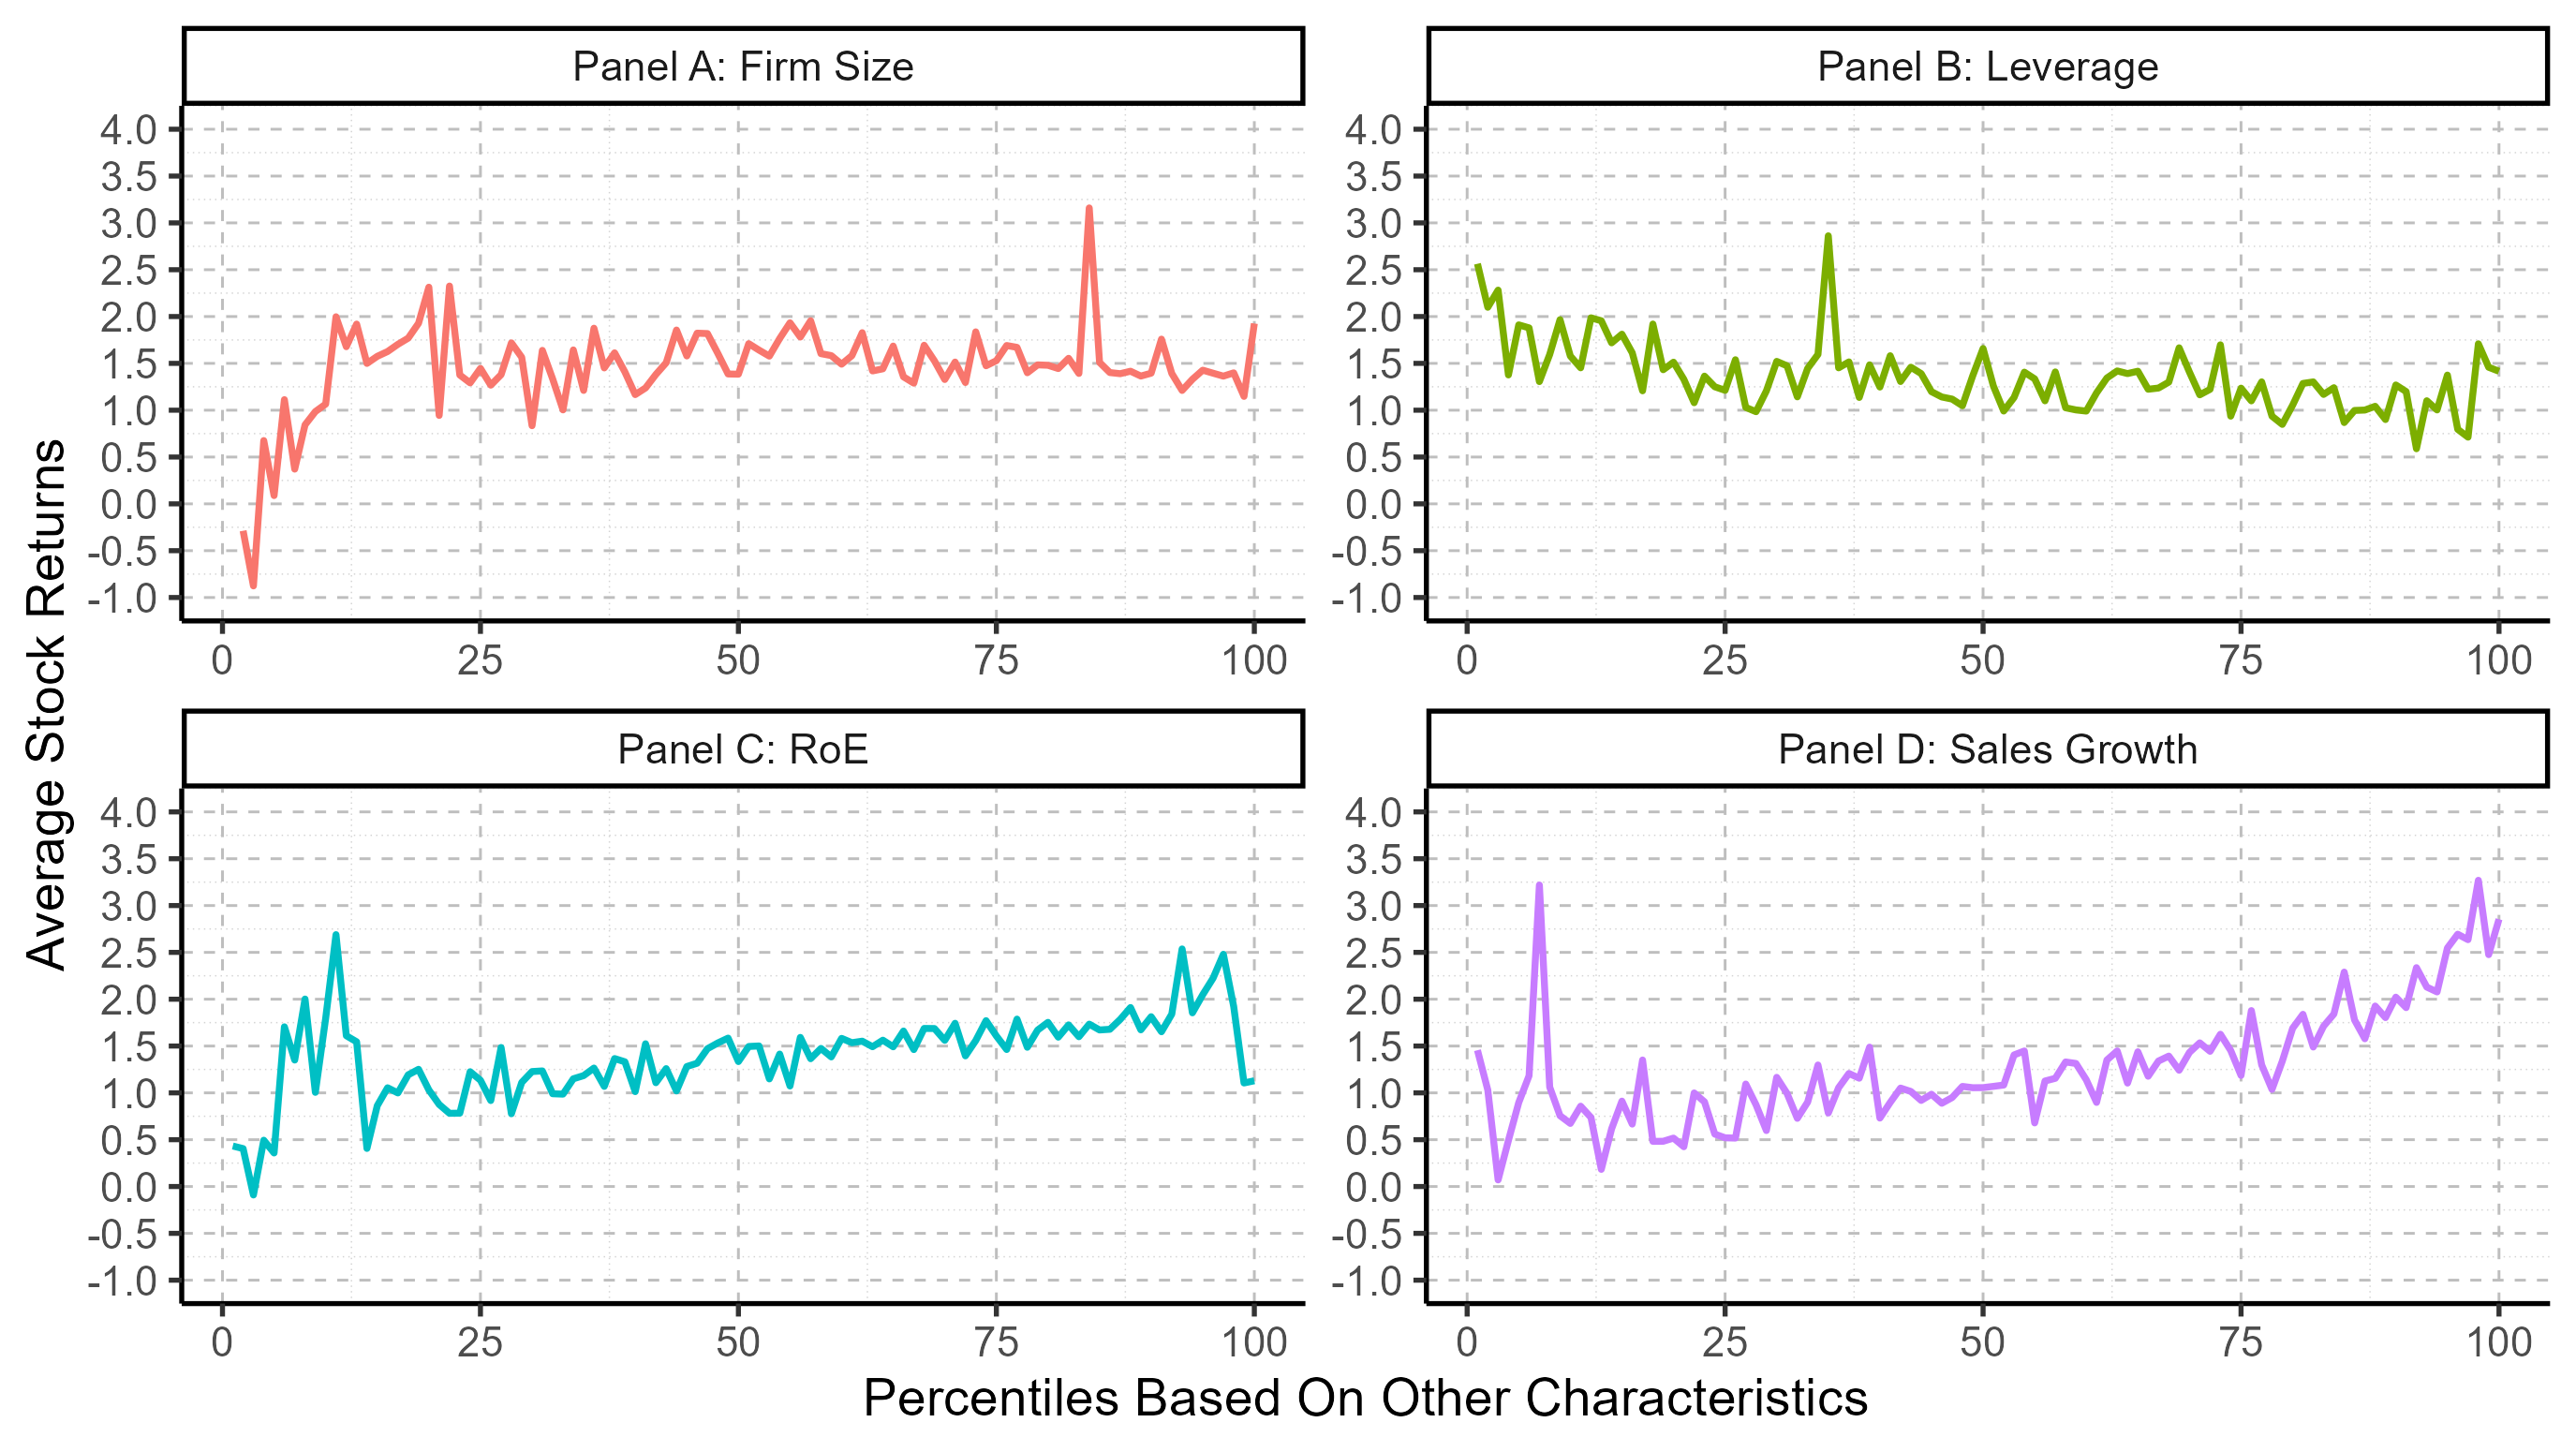
\includegraphics{image/others_percentile.png}
\label{fig: others_persentile}
\caption*{\footnotesize{This presents the average monthly stock returns in relation to different percentiles of various firms' characteristic indicators. Panel A depicts the average stock return in relation to firms' market capitalization, while Panel B illustrates the average stock return concerning firms' leverage. Panel C showcases the average stock return with respect to firms' profitability ROE, and Panel D presents the average stock return in connection with firms' growth in revenue.}}
\end{figure}

%%%%%%%%%%%%%%%%%%%%%%%%%%%%%%%%%%%%%%%%%%%%%%%%%%%%%%%%%
\subsection{Unexpected Climate Concern Index}
\label{sec: mcc}

In their study, \cite{ardia2022climate} develop the Media Climate Change Concerns Index (MCCC) at time $t$ by applying an increasing concave function, denoted as $h(x)$, to the average of source-specific climate change concerns after normalizing them for the same time period $t$. The formula is expressed as follows:

\begin{equation}
\label{mccc}
MCCC_t = h\left(\frac{1}{h}\sum^s_{s=1}nconcerns_{t,s} \right)
\end{equation}

It's noteworthy that several other studies have explored text-based methodologies for constructing similar indices, including \cite{engle2020hedging}, \cite{kapfhammer2020climate}, and \cite{faccini2021climate}. What distinguishes the MCCC index devised by \cite{ardia2022climate} is its ability to incorporate data from ten high-circulation media sources. This diversification is a notable strength, and it's worth highlighting that they update the index on a daily basis, allowing for aggregation at weekly and monthly frequencies, and enhancing its flexibility and timeliness. The historical trajectory of the monthly MCCC index is plotted in Figure \ref{fig: mccc}.

\begin{figure}[!ht]
\centering
\caption{\textbf{Media Climate Change Concerns Index}}
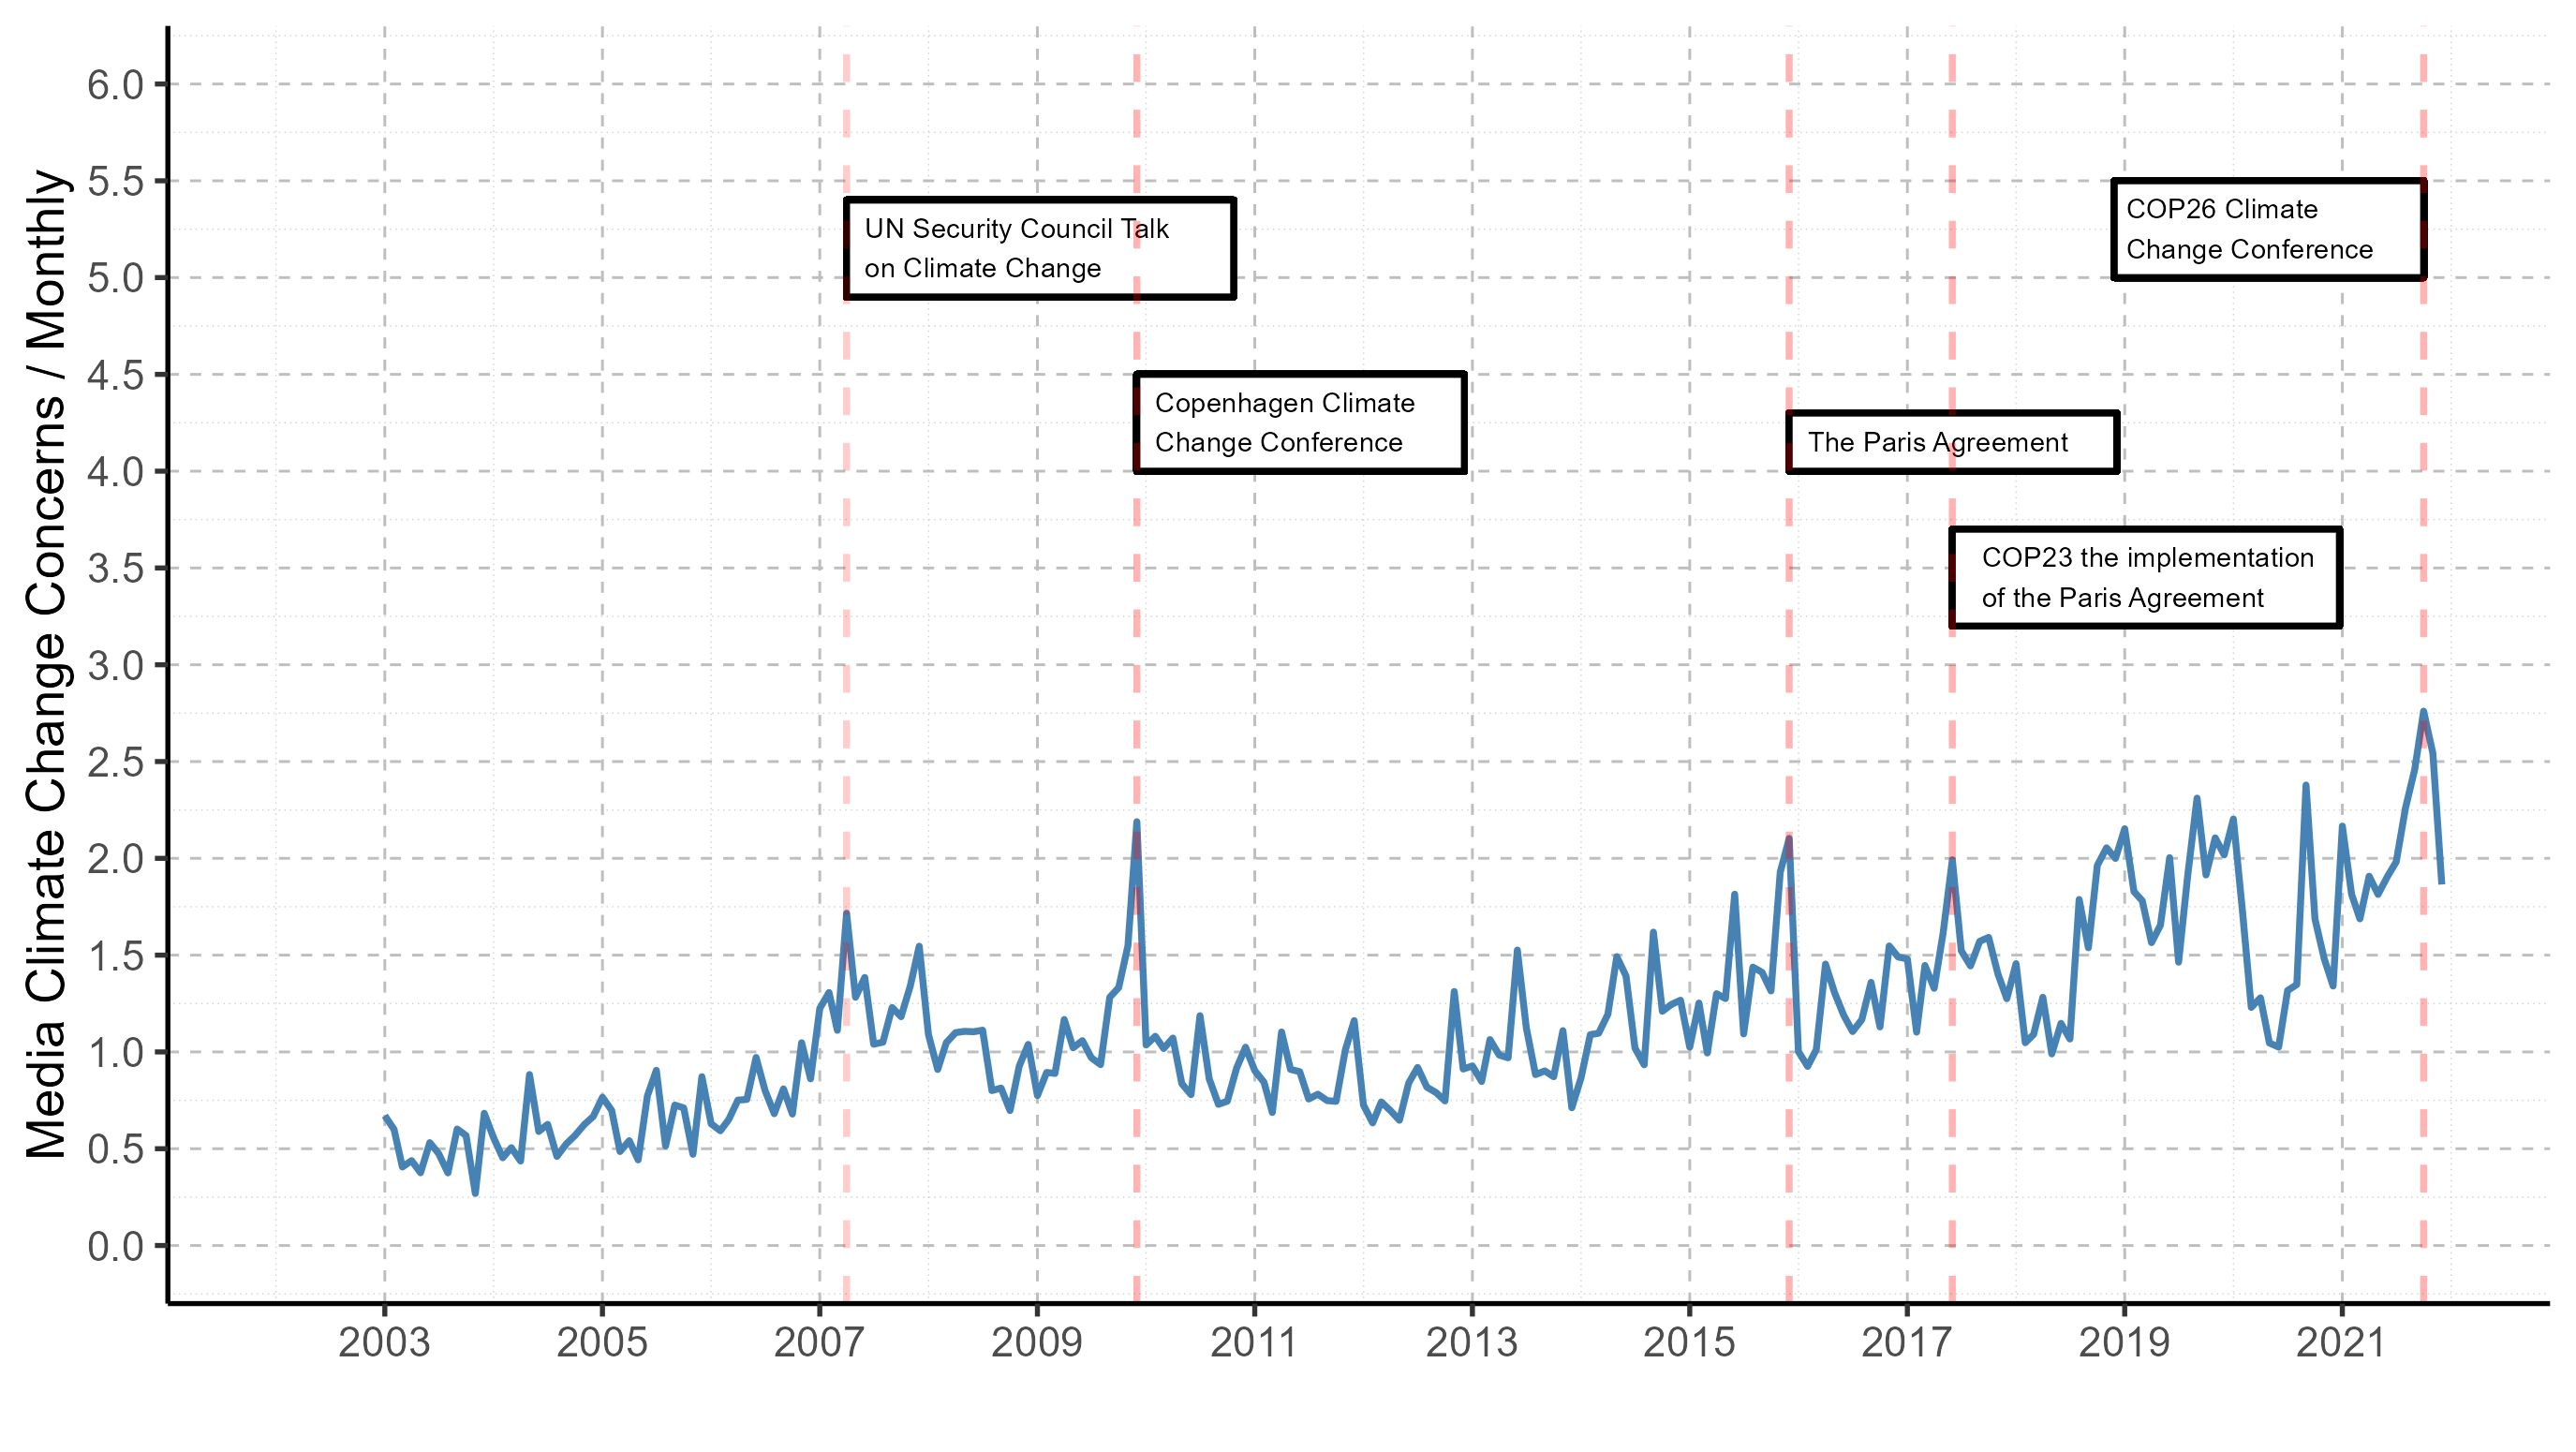
\includegraphics{image/mccc_plot.png}
\label{fig: mccc}
\caption*{\footnotesize{This figure presents the monthly MCCC (Media Climate Change Concerns) index from 2003 to 2021 together with the major climate-related events.}}
\end{figure}



\end{document}
